\documentclass[letterpaper, 12pt, parskip=full,DIV=10]{scrartcl}
% The next three lines are temporary, for todo notes, remove after notes are removed
%\documentclass[letterpaper, 12pt, parskip=full,]{scrartcl}
%\setlength{\marginparwidth}{4.5cm}
%\usepackage[top=2.5cm, bottom=2.5cm, left=1.5cm, right=5cm]{geometry}


\input{../preanalysis/template_MOW.sty}

\title{Battling the Coronavirus ``Infodemic'' Among Social Media Users in Africa}
%\subtitle{}
\author[1]{Molly Offer-Westort}
\author[2]{Leah R. Rosenzweig}
\author[3]{Susan Athey}
\affil[1]{Department of Political Science, University of Chicago; mollyow@uchicago.edu}
\affil[2]{Development Innovation Lab, University of Chicago}
\affil[3]{Stanford Graduate School of Business, Stanford University}
\date{\today}


\usepackage{titletoc}
\usepackage{siunitx}
\usepackage[splitrule]{footmisc}
\interfootnotelinepenalty=100000
\raggedbottom

\begin{document}%
\normalsize%
\maketitle%

%%%%%%%%%%%%%%%%%%%%%%%%%%%%%%%%%%%%%%%%%%%%
%FRONTMATTER
%%%%%%%%%%%%%%%%%%%%%%%%%%%%%%%%%%%%%%%%%%%%

\textbf{Author Contributions: }

\textbf{Competing Interest Statement: }\todo{add note with link to anonymized preanalysis plan}

\textbf{Classification:} \todo{Paste the major and minor classification here. Dual classifications are permitted, but cannot be within the same major classification.}

\textbf{Keywords (3-5):} Misinformation - covid - adaptive experiment

%% for nature human behavior:
%Main text – up to 5,000 words, excluding abstract, Methods, references and figure legends.
%Abstract – up to 150 words, unreferenced. 
%Display items – up to 8 items (figures and/or tables). 
%Article should be divided as follows: 
%Introduction (without heading) 
%Results (concise, focused account of the findings)
%Discussion
%Methods. ​

{\textbf{Abstract:}}
\begin{abstract} %150 words for nature human behavior (currently over by ~10)
%Big picture Q (1 sentence)
%Existing lit / state of lit - what we know / dont
%“We …” what this paper does (1)
%What we find (1-2)
%Implications (1)


% count: 159
What online interventions are effective at reducing willingness to share health misinformation during an ongoing global pandemic? Using an adaptive experiment with Facebook users recruited on the platform in Kenya and Nigeria, we tested 40 combinations of interventions with the goal of improving sharing discernment-- reducing intended sharing of false posts without adversely affecting true sharing-- of COVID-19 posts. We estimate precise null effects of flagging misleading posts and including related articles, which are used by social media platforms. Instead, providing tips for spotting misinformation and nudging users to think about the accuracy of media content improves sharing discernment. Tips leads to effects equivalent to a nearly 8\% reduction in intended sharing of false information, and nudging accuracy leads to a 4\% reduction.  %Both interventions are successful among some of the worst offenders, who intend to share more false news at baseline. % -- specifically men, users with lower digital literacy, and less scientific knowledge.
We also find significant differences in response to these treatments across users with different characteristics, indicating these interventions affect outcomes through separate mechanisms.  These low-cost scalable interventions may significantly improve the quality of information circulating online.

 
\end{abstract}

%\textbf{Significance statement:} %LR: I think we'll need to make this more specific once we have nailed down our specific contributions (beyond another study demonstrating that these things work)...
%Health misinformation can be deadly. Alongside the global coronavirus pandemic there has been an ``infodemic'' of rumors about the virus and hoax cures.  Which online interventions delivered via social media help to limit the spread of misinformation? We experimentally evaluated a slate of interventions to learn which are effective at reducing social media users' intentions to share false information about COVID-19 in Kenya and Nigeria. Warning labels on posts had little influence while accuracy prompts and tips had positive effects in both countries. The results suggest that platforms and policy makers may wish to consider implementing these low-cost scalable interventions to reduce the prevalence of misinformation. 


\clearpage

%%%%%%%%%%%%%%%%%%%%%%%%%%%%%%%%%%%%%%%%%%%%
%MAIN
%%%%%%%%%%%%%%%%%%%%%%%%%%%%%%%%%%%%%%%%%%%%

\section{Main}

\textcolor{red}{
Our contributions
\begin{enumerate}
\item Horse race among many interventions
\item Respondent works, not headline, and we learned two respondent that work especially well: FB vs accuracy. We can differentiate these to some extent. 
\item Measuring sharing channel adds nuance (helps us better understand how treatments work, and for whom?)\todo{LR: havent yet added this one in intro - will wait to see what we can say specifically}
\end{enumerate}
}

%Susan's comment:
%The introduction probably gets started too slowly, and doesn't spend enough time motivating the SPECIFIC contributions of this paper rather than the overall phenomenon.  It jumps around and goes from very general to very specific, kind of missing the middle.  Also there is little motivation of the adaptive experiment that tried lots of things.

%new main outline:
%1 par on big picture question / problem/ issue
%2nd par = “This paper…” (what it does, contribution, builds on work…)
%More on contributions [in context of existing literature]
%Paper’s methods
%More specifics/details on methods (“the empirical approach…” - (“see Methods for a detailed description”). “Our main analysis…”
%Limitations (cite later section after results)


% context / problem area --> more specific more quickly
Alongside the outbreak of the novel coronavirus (SARS-CoV-2), much of the world's population also experienced an ``infodemic''---the spread of misinformation related to the virus.  Before effective vaccines were developed and widely available, people across the globe looked to alternative sources for prevention techniques and remedies for the COVID-19 disease. In Nigeria, multiple people were hospitalized for chloroquine poisoning following statements by former president Trump suggesting the medication could be used to treat COVID-19 \citep{busari2020nigeria}. In Iran, dozens of people died from alcohol poisoning after ingesting methanol supposedly due to the rumor that alcohol could prevent coronavirus \citep{haghdoost2020alcohol}. %Particularly in contexts with weak healthcare systems, the uncertainty over how to combat COVID-19 infection may have been particularly daunting and the search for remedies that much more urgent. 
Understanding how to slow the spread of false ``cures'' may have life-saving consequences. % too much?
%LR: I cut to 5 sentences - I initially just had the nigeria example and cut iran but it puts a fine point on *deadly* consequences..


% our study - what we do / contribute
This paper focuses on these particularly dangerous pieces of COVID-19 misinformation -- hoax ``cures'' -- and tests numerous online interventions designed to curb sharing of these falsities on social media, while not adversely affecting the sharing of true information on COVID-19 prevention techniques.  This study began in February 2021 before vaccines were widely available. Using targeted Facebook advertisements, we recruited a sample of social media users living in Kenya and Nigeria, two of the three largest Facebook markets in sub-Saharan Africa \citep{world-population-reviewfacebook}. Using a Facebook Messenger chatbot,  we engaged participants in a survey experiment that recruited and kept these social media users on the platform where they would naturally engage with similar media posts.  Participants answered survey questions and were randomized into different treatments delivered by the Messenger chatbot. 

% sharing = outcome of interest - also measure BY CHANNEL

Our main outcome of interest is intended sharing discernment: whether respondents indicate wanting to share true but not false posts. We focus on sharing rather than belief, since exposure can further false narratives through resharing even if it doesn't affect an individual's belief, and because exposure to COVID-19 misinformation can cause lower adoption of preventative behaviors \citep{bursztyn2022opinions}. In addition to measuring participant's intentions to share both true and false COVID-19 posts, we measured \textit{how} they wanted to share each post -- either publicly on their Timeline or privately on Messenger. \textcolor{red}{We analyze/examine sharing intentions by post type/veracity as well as by sharing channel in order to understand users' sharing preferences at baseline and post treatment.}\todo{LR: maybe add another sentence here on specific response function in order to avoid going through setup in results section?}


% CUT SHARING LIT REVIEW: 
% Misinformation can have harmful effects, regardless of the motivation for sharing: there is suggestive evidence that the spread of misinformation is correlated with behavior. One study analyzed more than 100 million Twitter posts worldwide and found a correlation between waves of unreliable information prior to a rise in COVID-19 infections \citep{gallotti2020assessing}.  One study of Fox News viewers in the US finds that greater exposure to COVID-19 misinformation is associated with lower adoption of preventative behaviors \citep{bursztyn2022opinions}.
 %Randomized controlled trials also find that exposure to COVID-19 misinformation lowers intentions to engage in physical distancing among a convenience sample of German university students \citep{pummerer2022conspiracy} and intentions get the vaccine among nationally representative samples in the US and UK \citep{loomba2021measuring}. 


% learning phase + interventions
Towards the goal of understanding what works to improve sharing discernment we first ran a learning phase using a multi-factorial adaptive design to compare a set of 40 treatments against each other and control.  We examine interventions delivered to both the individual user, such as tips for spotting fake news, training videos, and nudges; as well as treatments delivered on specific posts, such as flags or warning labels pinned on the article of interest. We differentiate between these types of interventions because they vary in their cost and scalability. This design allowed us to identify which respondent-level and headline-level treatments were most effective at reducing intentions to share false information without adversely affecting true sharing.\footnote{Table \ref{tab:treatments} in the Supplementary Information (SI) describes all of the interventions we tested.} \textcolor{red}{We differentiate between these types of interventions because they vary in their cost and scalability, specific post flags require resource-intensive fact checking sources to keep up to pace with the generation of new misinformation.}\todo{LR: I moved rest of this to discussion/conclusion}

Our adaptive algorithm optimized for treatments that improved a response function that weighed intention to share a false post twice as (negatively) as wanting to share a true post (positively).\footnote{In the next section we also show results of the interventions disaggregated by post type and sharing channel.} The adaptive design sequentially assigned treatment probabilities to privilege assignment to the most effective interventions, and minimized assignment to ineffective or counter-productive interventions.  \textcolor{blue}{[Still to add here: more specifics on response funct?,  benefit to adaptivity...]} Traditional randomized experiments are often limited in the number of interventions they can test due to power considerations, but our adaptive design allows us to sort through numerous interventions. \todo{I can add a lot of the design stuff in for the next edit, and then make consistent/remove duplication across here, results, and methods.}


% mention learning phase + eval. phase --> contribution = testing many interventions at once!


% eval phase -  we find: respondent  > headline.  tips + accuracy (as others have found) - but we're able to dig into heterogeneity/optimal policy to say more about how the types of people differ for whom one of these policies is better over the other --> provides greater insights into the different mechanisms/processes through which these interventions operate.

After identifying the two most successful headline-level and respondent-level interventions from the adaptive learning phase,  we ran an evaluation phase to [identify the optimal policy/compare against each other and control].  With a new sample of Facebook users from Kenya and Nigeria in the evaluation phase, we tested  factcheck labels and related articles headline-level treatments, and tips for spotting misinformation \citep{guessetal2020digital} and an accuracy nudge \citep{pennycook2021shifting} for the respondent-level treatments. We find that the headline-level interventions do not perform better than control, and estimate precise null effects for these treatments. We do, however, see that tips and the accuracy nudge improve sharing discernment.  \textcolor{blue}{[ADD specific findings re. heterogeneity / what we can say about distinguishing btw accuracy and tips...]} By exploring heterogeneity in response to treatment we are able to say more specifically which types of users do best under which treatment/who should be targeted with each. The findings provide further evidence that these interventions are not perfect substitutes, perhaps because they operate through different mechanisms, and there are benefits to targeting users with different characteristics with tips over accuracy and vice versa. % say this better



%intention - behavior gap - concerns of experimenter demand bias. survey exp. not field exp. 

% our contributions / benefit over other similar studies - in context of general limitations re. external validity

\textbf{[LR: will make last 4 paragraphs our contribution + lit review to serve that end]}

\todo{LR: summarize limitations here and then put longer discussion in limitations subsection in discussion?} 
This study, like others focused on online misinformation, faces several limitations related to external validity. First, our goal is to identify interventions that are effective among the population of social media users in Kenya and Nigeria. We are limited, however, in our recruitment methods to engaging with those who clicked on our Facebook ads to participate in the study.  Recruiting actual social media users on the platform is an improvement beyond convenience samples, laboratory experiments, and opt-in survey panels.  We cannot say, however, how users who decided to participate in our study differ on unobservables to the general population of Facebook users in these countries. Importantly, this study brings comparative data to this global question which is most often studied using samples recruited from Qualtrics, Lucid, and MTurk in North America.  

% survey experiment 
Second, interacting with participants of a study and delivering interventions in the course of a survey experiment is an imperfect proxy for understanding how users would react to real interventions delivered on the platform.  Though still artificial, our approach of delivering the survey and interventions through a Facebook Messenger chatbot provides greater realism than interventions delivered on other platforms like Qualtrics.  The nature of our survey experiment means that participants were aware they were part of a study (rather than an on-platform field experiment, for example,  where consent may be waived by IRB or implicitly provided when users agree to the terms and conditions). Therefore, it is possible that participants' responses could be driven by experimenter demand effects. The validity of our findings would be at risk if participants gleaned the intention of the study and adjusted their responses to match what they thought the researchers wanted to hear, rather than reflecting how they truly believed or wanted to behave.  \textcolor{red}{[TK (for now referenced on p.15): Later we presents tests that suggest our results are not wholly driven by experimenter demand bias.]} %\todo{MOW: not in here yet, currently referenced on p. 14. }

%sharing outcome 
Finally, misinformation studies that focus on sharing behavior as the main outcome of interest are constrained by ethical considerations of not wanting to contribute to the ecosystem of misinformation by allowing survey participants to \textit{actually share} false posts. This study,  like most others, instead use measures of sharing \textit{intentions}.  While scholars have found that intentions are correlated with online sharing behavior \citep{mosleh2020self}, measuring intentions rather than actual behavior remains a main limitation of scholarship in this area.  In this study, we directly ask participants ``Do you want to share this post on your timeline/on Messenger?,'' rather than phrasing it as a hypothetical question. We simultaneously told participants not to share the post now, but they would be able to do so at the end of the study. When we debriefed respondents at the end of the study, we told them which posts they saw were false and explained that was why they could not share those posts. We gave participants an opportunity to share the true posts they had said they wanted to share. \todo{check this is correlated with true sharing intentions.} A unique contribution of this study is that for each post (true and false), we asked participants if they wanted to share it on Timeline (public to their friends on Facebook) or on Messenger (a direct private message). We observe variation in sharing preferences by channel that suggest participants are discerning in their stated sharing intentions for true and false posts at baseline. \todo{A full page of limitations feels like a bit much in the first 4 substantive pages of the paper.}

% LR ADD NEXT TIME: \textcolor{blue}{Some studies do not measure or analyze the reactions to false posts -- though important without also measuring treatment effects on sharing of true posts, they are unable to determine whether the intervention makes people overall more skeptical or improves discernment \citep{modirrousta2022effective}.}


%This study aimed to understand what online interventions might be effective at curbing the spread of hoax COVID ``cures'' on social media among users in two African countries. Several challenges exist in trying to answer this question without access to on-platform experimentation. 



% specific research questions / contributions - play up design and the more nuanced targeting questions we ask/answer
% maybe use this par as outline par - if results section comes next - outline subsections of results...

\textcolor{blue}{\todo{LR: will edit this once we nail down results section}
This paper investigates several important questions.  Do social media users have different preferences for how they share true and false posts about COVID-19? Can we identify interventions that are effective at reducing the sharing of false information, without adversely affecting sharing of true information? We also explore whether there are benefits to policy targeting from two perspectives. First, we analyze which recipients should be targeted with interventions. Second, we observe whether particular interventions should be designated for certain types of users and not for others.  This study is able to take a more comprehensive approach toward subgroup analysis by exploring who shares the most misinformation at baseline and who is most affected by treatment looking at covariates academic studies have found to be significant predictors, as well as characteristics platforms collect on users. With the goal of minimizing the spread of misinformation in the online information ecosystem, we quantify the best approach in this setting and offer lessons for other contexts.}




%%%%%%%%%%%%%%%%%%%%%%%%%%%%%%%%%%%%%%%%%%%%
%RESULTS
%%%%%%%%%%%%%%%%%%%%%%%%%%%%%%%%%%%%%%%%%%%%

\section{Results}
\paragraph{Study sample}
We conducted this study with social media users in Kenya and Nigeria, two major English-language hubs of online communication in East and West Africa, respectively. We recruited social media users 18 years and over in these countries through targeted Facebook advertisements \citep[see our advertisement in Figure~\ref{fig:recruitment} in the SI; for further details on targeted recruitment on Facebook, see][]{Rosenzweig_2020}.  Users who clicked on our ads were prompted to start a conversation with our research page's Messenger chatbot. The chatbot serves both to collect survey responses and to deliver experimental interventions. 

The study was conducted in two stages, each with unique respondents: a ``learning'' stage, with 4,553 social media users, and an ``evaluation'' stage, with 10,681 social media users. In Supplementary Table~\ref{tab:demographics} we report sample characteristics and comparison to nationally representative Afrobarometer surveys. 
%Supplementary Table~\ref{tab:cov_long} reports demographic, social, and political questions collected during the chatbot conversation which are used for adjustment in both the learning and evaluation stages. 

\paragraph{Primary outcomes}
We operationalized sharing discernment using a combined response measure of sharing intentions. Both before and after treatment, participants in the experiment were shown a series of real social media posts about COVID-19 cures, treatments, and preventative best practices. For each stimuli, users were separately asked whether they would like to share the stimuli through two channels: on Facebook Messenger and on their Facebook timeline. 

Our pre-specified combined response measure is a weighted sum of times users said they would like to share true and misinformation stimuli over each channel. As our objective is to learn treatments that will decrease sharing of false information while not overly harming sharing of true information, intentions to share false stimuli are given a weight of -1, and intentions to share true stimuli are given a weight of 0.5 in this measure. More details on this measure are provided in Methods Section~\ref{section:measures}. 

We also report results for both types of stimuli separately: we report the proportion of true and false stimuli respondents reported intending to share, across either Messenger or timeline, as well as disaggregated by sharing channel.  


\paragraph{Learning and evaluation stages}
We designed the learning stage to compare a large range of treatment conditions, and learn which of them were most effective on our pre-specified combined response measure.  We considered two classes of interventions: seven respondent-level interventions and four headline-level interventions. The respondent-level interventions included behavioral nudges and trainings targeted to the participants themselves: tips and trainings to spot false news (from Facebook, AfricaCheck, and a BBC video), an emotion suppression prompt, an accuracy nudge, and a pledge that participants took to keep their family and friends safe. The headline-level interventions were applied to the headlines or posts themselves: a flag for articles that had been fact checked by third-party websites, links to further information, or accompanied by additional related articles or countering information from a validated source such as the WHO. Table~\ref{tab:treatments} in the Supplementary Information (SI) describes all of the interventions we tested. %Section~\ref{appendix:learning} in the SI discusses learning stage design and results. 
We used a multi-factorial experimental design where each class of intervention was treated as a separate multi-level factor, with a baseline control condition. 

To assign treatment in the learning stage of our study, we used a contextual adaptive assignment algorithm, a version of balanced linear Thompson sampling \citep{dimakopoulou2017estimation,dimakopoulou2019balanced},  by which we updated treatment assignment probabilities based on the observed history of treatment, response, and covariates. 
Under Thompson sampling, treatment is assigned according to the Bayesian posterior probability that each treatment is associated with the highest mean response. In linear Thompson sampling, this is generalized to allow the outcome to be a linear function of covariates. 

This adaptive design allowed us to continue to learn which treatment was best, while reducing the probability that users were assigned to ineffective or harmful interventions. \textcolor{blue}{One methodological contribution of this study is to demonstrate the benefit of using adaptive experiments to learn more quickly and avoid sending poorly performing treatments - that may also backfire and increase sharing of misinformation - to more respondents, as conventional experiments with static treatment assignment probabilities do.} The inclusion of treatment-covariate interactions in the assignment model allows for the possibility that different interventions may be most effective for users with different covariate profiles. 
Figure~\ref{fig:learning_cumulative} in the SI illustrates the development of cumulative assignment under our assignment algorithm. 
%In our version of linear Thompson sampling, we treated respondent-level and headline-level treatments as separate treatment factors, each with a baseline control condition.

%\textcolor{red}{[ADD par. on how much (intended) false sharing we avoided using an adaptive design - can think about impact in context of studies that allow for actual sharing (e.g. on platform) or that seek to move intentions for behaviors, such as studies that have experimentally resulted in lower willingness to get vaccinated \citep{loomba2021measuring}. }
%\textbf{[figure of mean response across all learning phase treatments?]} 

From the data in the learning stage, we selected two ``best'' treatments each from the respondent-level and headline-level classes. 
These were the two treatments associated with the highest estimated mean responses in each class separate from control, as measured on our combined response outcome. %, as estimated using the estimator described in Equation~\ref{eq:scores_learning} with our combined response measure as the outcome. 
These treatments were the accuracy nudge and Facebook tips (respondent-level) and factcheck and related articles (headline-level); examples of each are presented in the Methods Section, Figure~\ref{fig:4treatments}. 

%\paragraph{Evaluation stage}
In the evaluation stage, we compared these most effective interventions to the control to obtain precise estimates of their effects. Treatment was assigned with equal probability to each of these or to an optimal contextual policy, which assigned to each user the respondent-level treatment predicted to be best for them conditional on their covariate profile. We included only the two ``best'' respondent-level treatments in this optimal policy, as our results from the learning stage suggested that headline-level treatments at best improved only minimally over control (Figure~\ref{fig:learning_estimates} in the SI reports estimated response in the learning stage). The following results are all based on data analyzed from the evaluation stage.\footnote{{
To learn a contextual policy, we fit the augmented inverse probability weighted estimator described in Equation~\ref{eq:scores_learning} to the learning data. From this model, we predicted responses for each covariate profile in the evaluation stage under counterfactual treatment conditions. The contextual policy assigned to each user the treatment associated with the highest predicted response, conditional on their covariates. In the main results here, we report results with respect to a policy learned on the false sharing outcome measure only, and include as possible treatments only the two ``best'' respondent-level treatments included in our evaluation.  % i think this sentence was already said above?
 
Prior to collecting the evaluation data, we fit a contextual policy using the combined response measure, including a broader range of respondent-level treatments. However, as false sharing intentions are more responsive to treatment, the inclusion of true sharing intentions in the measure adds noise. We report outcomes for the policy learned on the combined response measure in Section~\ref{appendix:learning} in the SI. 
}}

\paragraph{Discernment under control}
Under the control condition, we see that users exhibit discernment in what types of stimuli they intend to share and through which channels. Overall, users report greater intentions to share true stimuli %(65.1, SE = 0.8) 
as compared to false stimuli %(44.2, SE = 0.9) 
on any channel (difference = 20.9 pp, SE = 0.9).  Users are also more likely to want to share true stimuli publicly on their timeline %(59.3, SE = 0.9) 
as compared to by private message %(56.1, SE = 0.9)
(difference = 3.1 pp, SE = 0.7), but the reverse is true for false stimuli (difference = -2.9 pp, SE = 0.6). The data suggest that even at baseline participants are able to differentiate between true and false posts to some extent, and, when they do indicate wanting to share false posts, they make different decisions about how to share them as compared to true posts. 
%This discernment by channel demonstrates that even when users intend to share false stimuli, they are making different decisions about the way in which they share it. 

We also find that covariates are highly predictive of heterogeneity in baseline sharing behaviors among users. Understanding baseline heterogeneity in sharing behavior helps us to identify the greatest culprits of sharing misinformation.  We focus on several key variables for examining heterogeneity, as well as for targeting interventions: age, gender, political allegiance, digital literacy, and scientific knowledge. We focus on these pre-registered variables as they may already be measured by social media platforms (age, gender) or are of theoretical interest in social scientific research (political allegiance, digital literacy, and scientific knowledge).

Our data suggest that under control, older subjects, those aligned with the ruling party, participants with low digital literacy and those with low scientific knowledge have relatively lower valued outcomes on our combined response measure, indicating relatively higher false sharing intentions and/or lower true sharing intentions (see Table~\ref{tab:heterogeneity_control}).

\begin{table}[H]
   \centering
\resizebox{\textwidth}{!}{ 
\begin{tabular}{lccccccc}
&    & \multicolumn{3}{c}{\textbf{False}} & \multicolumn{3}{c}{\textbf{True}} \\
& \textbf{Combined}& Any sharing & Messenger & Timeline & Any sharing & Messenger & Timeline \\
 \cmidrule(lr){2-2}  \cmidrule(lr){3-5}  \cmidrule(lr){6-8}
\multicolumn{4}{l}{\textbf{  Overall control mean}} \rule{0pt}{1.2\normalbaselineskip} \\
 & \num{-0.391} & \num{0.442} & \num{0.395} & \num{0.369} & \num{0.651} & \num{0.561} & \num{0.593}\\
 & (\num{0.027}) & (\num{0.009}) & (\num{0.008}) & (\num{0.008}) & (\num{0.008}) & (\num{0.009}) & (\num{0.009}) \\
 \hline
\multicolumn{4}{l}{\textbf{Age}} \rule{0pt}{1.2\normalbaselineskip} \\
\hspace{1em} Below median  & \num{-0.484} & \num{0.457} & \num{0.413} & \num{0.374} & \num{0.632} & \num{0.548} & \num{0.562}\\
\hspace{1.5em} (n = 5,412) & (\num{0.035}) & (\num{0.012}) & (\num{0.012}) & (\num{0.011}) & (\num{0.012}) & (\num{0.013}) & (\num{0.012})\\
\hspace{1em} Above median & \num{-0.295} & \num{0.425} & \num{0.380} & \num{0.361} & \num{0.670} & \num{0.575} & \num{0.624}\\
\hspace{1.5em} (n = 5,271)  & (\num{0.040}) & (\num{0.012}) & (\num{0.012}) & (\num{0.012}) & (\num{0.012}) & (\num{0.012}) & (\num{0.012})\\
\cmidrule(lr){2-8}
\hspace{1em} Difference& \num{-0.189}*** & \num{0.032}+ & \num{0.033}* & \num{0.012} & \num{-0.038}* & \num{-0.028} & \num{-0.062}***\\
 & (\num{0.054}) & (\num{0.017}) & (\num{0.017}) & (\num{0.016}) & (\num{0.017}) & (\num{0.018}) & (\num{0.017})\\
\multicolumn{4}{l}{\textbf{Gender}}  \rule{0pt}{1.2\normalbaselineskip}\\
\hspace{1em} Not male   & \num{-0.356} & \num{0.400} & \num{0.362} & \num{0.327} & \num{0.611} & \num{0.512} & \num{0.543}\\
\hspace{1.5em}  (n = 5,050)& (\num{0.037}) & (\num{0.012}) & (\num{0.012}) & (\num{0.011}) & (\num{0.012}) & (\num{0.013}) & (\num{0.012})\\
\hspace{1em} Male & \num{-0.422} & \num{0.478} & \num{0.427} & \num{0.404} & \num{0.687} & \num{0.605} & \num{0.637}\\
\hspace{1.5em}  (n = 5,633)  & (\num{0.038}) & (\num{0.012}) & (\num{0.012}) & (\num{0.012}) & (\num{0.011}) & (\num{0.012}) & (\num{0.012})\\
\cmidrule(lr){2-8}
\hspace{1em} Difference  & \num{0.067} & \num{-0.077}*** & \num{-0.077}*** & \num{-0.077}*** & \num{-0.076}*** & \num{-0.076}*** & \num{-0.076}***\\
 & (\num{0.053}) & (\num{0.017}) & (\num{0.017}) & (\num{0.017}) & (\num{0.017}) & (\num{0.017}) & (\num{0.017})\\
\multicolumn{4}{l}{\textbf{Political allegiance}} \rule{0pt}{1.2\normalbaselineskip}\\
\hspace{1em} Not aligned & \num{-0.333} & \num{0.415} & \num{0.366} & \num{0.340} & \num{0.629} & \num{0.537} & \num{0.563}\\
\hspace{1.5em} (n = 7,570)  & (\num{0.032}) & (\num{0.010}) & (\num{0.010}) & (\num{0.010}) & (\num{0.010}) & (\num{0.011}) & (\num{0.010})\\
\hspace{1em} Aligned & \num{-0.532} & \num{0.504} & \num{0.469} & \num{0.434} & \num{0.704} & \num{0.621} & \num{0.664}\\
\hspace{1.5em} (n = 3113) & (\num{0.050}) & (\num{0.016}) & (\num{0.016}) & (\num{0.015}) & (\num{0.015}) & (\num{0.016}) & (\num{0.016})\\
 \cmidrule(lr){2-8}
\hspace{1em} Difference & \num{0.199}*** & \num{-0.089}*** & \num{-0.089}*** & \num{-0.089}*** & \num{-0.075}*** & \num{-0.075}*** & \num{-0.075}***\\
 & (\num{0.059}) & (\num{0.019}) & (\num{0.019}) & (\num{0.019}) & (\num{0.018}) & (\num{0.018}) & (\num{0.018})\\
\multicolumn{4}{l}{\textbf{Digital literacy index }}  \rule{0pt}{1.2\normalbaselineskip}\\
\hspace{1em} Below median & \num{-0.536} & \num{0.495} & \num{0.448} & \num{0.421} & \num{0.674} & \num{0.587} & \num{0.620}\\
\hspace{1.5em}  (n = 5,443) & (\num{0.038}) & (\num{0.012}) & (\num{0.012}) & (\num{0.012}) & (\num{0.011}) & (\num{0.012}) & (\num{0.012})\\
\hspace{1em} Above median  & \num{-0.240} & \num{0.385} & \num{0.343} & \num{0.313} & \num{0.627} & \num{0.535} & \num{0.564}\\
\hspace{1.5em}  (n = 5,240) & (\num{0.037}) & (\num{0.012}) & (\num{0.012}) & (\num{0.011}) & (\num{0.012}) & (\num{0.013}) & (\num{0.013})\\
\cmidrule(lr){2-8}
\hspace{1em} Difference & \num{-0.296}*** & \num{0.110}*** & \num{0.106}*** & \num{0.108}*** & \num{0.048}** & \num{0.052}** & \num{0.056}**\\
 & (\num{0.053}) & (\num{0.017}) & (\num{0.017}) & (\num{0.016}) & (\num{0.017}) & (\num{0.018}) & (\num{0.017})\\
\multicolumn{4}{l}{\textbf{Scientific knowledge index}} \rule{0pt}{1.2\normalbaselineskip} \\
\hspace{1em} Below median & \num{-0.445} & \num{0.458} & \num{0.414} & \num{0.385} & \num{0.658} & \num{0.563} & \num{0.597}\\
\hspace{1.5em}   (n = 5,677) & (\num{0.036}) & (\num{0.012}) & (\num{0.012}) & (\num{0.011}) & (\num{0.012}) & (\num{0.012}) & (\num{0.012})\\
\hspace{1em} Above median & \num{-0.330} & \num{0.422} & \num{0.377} & \num{0.347} & \num{0.643} & \num{0.559} & \num{0.587}\\
\hspace{1.5em}  (n = 5,006)  & (\num{0.040}) & (\num{0.013}) & (\num{0.012}) & (\num{0.012}) & (\num{0.012}) & (\num{0.013}) & (\num{0.013})\\
\cmidrule(lr){2-8}
\hspace{1em} Difference  & \num{-0.115}* & \num{0.036}* & \num{0.036}* & \num{0.038}* & \num{0.015} & \num{0.004} & \num{0.010}\\
 & (\num{0.054}) & (\num{0.017}) & (\num{0.017}) & (\num{0.016}) & (\num{0.017}) & (\num{0.018}) & (\num{0.017})\\
   \end{tabular}}
   \caption{\textbf{Heterogeneity in response under the control condition by selected covariates.} Estimates are of mean response under the control condition, and are produced from an augmented inverse probability weighted estimator, as described in Section~\ref{section:estimation}, within specified subgroups. For contrasts only, under two-sided hypothesis tests: \textsuperscript{+} $p<0.1$, \textsuperscript{*} $p < 0.05$, \textsuperscript{**} $p < 0.01$, \textsuperscript{***} $p < 0.001$.}
\label{tab:heterogeneity_control}
\end{table}


\begin{figure}[H]
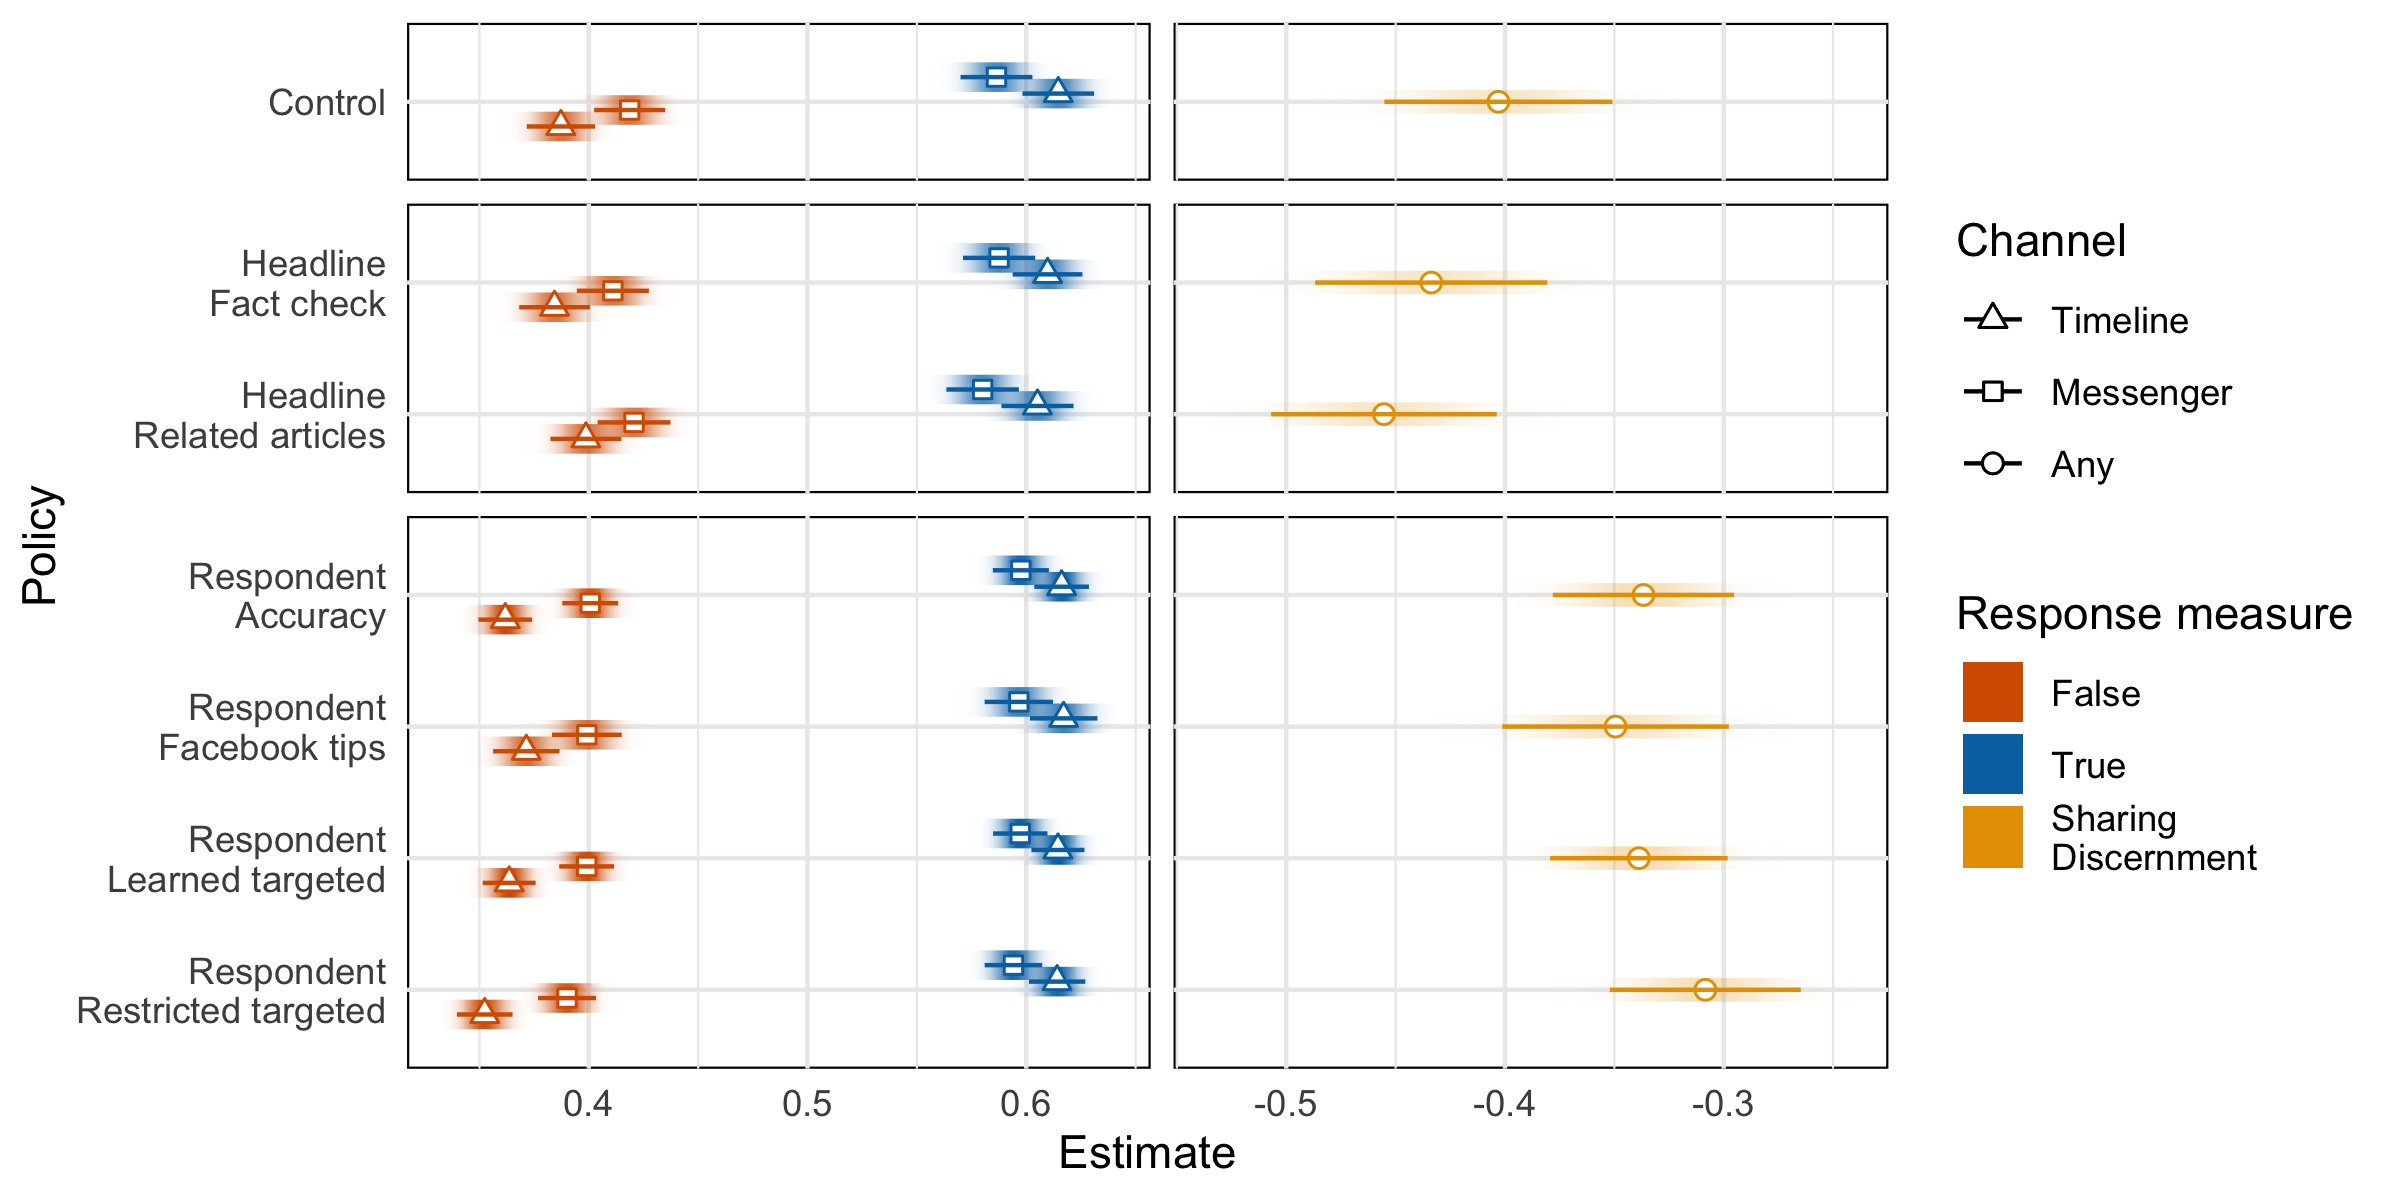
\includegraphics[width = \textwidth]{../analysis/figures/evaluated_scores_all.png}
\caption{\textbf{Response estimates.} Response measures are average intention to share true and false stimuli over either channel, and a combined response measure, reported in Section~\ref{section:measures}. Estimates are produced from an augmented inverse probability weighted estimator, as described in Section~\ref{section:estimation}.}
\label{fig:main_results}
\end{figure}


\paragraph{Main treatment effects}
Table~\ref{tab:main_results} shows tests of our pre-specified comparisons of each evaluated treatment condition against the control. We report results for the evaluation phase under the pre-registered combined response function, as well as disaggregated by any intention to share false and true stimuli by either channel, and false and true sharing intentions by each channel. Our objective is to decrease intentions to share false information, while minimizing negative effects on intentions to share true information. To this end, an effective intervention would result in positive treatment effects for our combined response function, negative treatment effects on false sharing, and positive or neutral treatment effects on true sharing; we pre-registered one-sided hypothesis tests with respect to these treatment effects. %FN last part?

The two headline-level treatments are not effective at decreasing sharing of false stimuli while maintaining rates of sharing true stimuli. The related articles treatment directionally increases intention to share false stimuli as compared to control, although this estimate is not statistically distinguishable from zero at conventional significance levels. The factcheck treatment is associated with a decrease of 0.5 pp (SE = 1.2) in false sharing intentions as compared to control; the effect would need to be nearly four times as large with the same degree of uncertainty for the confidence interval to exclude zero.  % next round: add more on how to interpret / quantify relative pp change in treatment effects

The respondent-level treatments, however, are effective. The Facebook tips and accuracy nudge treatments increase the combined response measure by 4.6 pp (SE = 3.5) and 6.0 pp (SE = 3.2) relative to control, respectively. These effects are driven by decreases in false sharing of 3.3 pp (SE = 1.1) for Facebook tips and 2.0 pp (SE = 1.0) for the accuracy nudge. Effects on true sharing are not distinguishable from zero at conventional significance levels for either treatment. 
These interventions speak to the debate on whether misinformation spreads because people are not paying attention or people do not have skills or information to spot it \citep{ecker2022psychological}. 

\begin{table}[H]
\centering
\resizebox{\textwidth}{!}{ 
\begin{tabular}{lccccccc}
&    & \multicolumn{3}{c}{\textbf{False}} & \multicolumn{3}{c}{\textbf{True}} \\
& \textbf{Combined}& Any sharing & Messenger & Timeline & Any sharing & Messenger & Timeline \\
 \cmidrule(lr){2-2}  \cmidrule(lr){3-5}  \cmidrule(lr){6-8}
\multicolumn{4}{l}{\textbf{Headline treatment effects}} \rule{0pt}{1.2\normalbaselineskip}\\                            
\hspace{1em} Factcheck   & \num{-0.032} & \num{-0.005} & \num{-0.004} & \num{-0.005} & \num{-0.003} & \num{-0.001} & \num{-0.012}\\
 & (\num{0.036}) & (\num{0.012}) & (\num{0.011}) & (\num{0.011}) & (\num{0.011}) & (\num{0.012}) & (\num{0.012})\\
 \hspace{1em} Related articles   & \num{-0.054} & \num{0.008} & \num{0.002} & \num{0.009} & \num{-0.019} & \num{-0.012} & \num{-0.021}\\
 & (\num{0.035}) & (\num{0.012}) & (\num{0.011}) & (\num{0.011}) & (\num{0.011}) & (\num{0.012}) & (\num{0.012})\\
\multicolumn{4}{l}{\textbf{Respondent treatment effects}}\rule{0pt}{1.2\normalbaselineskip} \\                            
\hspace{1em} Accuracy  & \num{0.060}* & \num{-0.020}* & \num{-0.018}* & \num{-0.026}** & \num{-0.001} & \num{0.005} & \num{-0.011}\\
 & (\num{0.032}) & (\num{0.010}) & (\num{0.010}) & (\num{0.009}) & (\num{0.010}) & (\num{0.010}) & (\num{0.010})\\
\hspace{1em} Facebook tips   & \num{0.046}+ & \num{-0.033}** & \num{-0.029}** & \num{-0.030}** & \num{-0.016} & \num{-0.005} & \num{-0.022}\\
 & (\num{0.035}) & (\num{0.011}) & (\num{0.011}) & (\num{0.010}) & (\num{0.011}) & (\num{0.012}) & (\num{0.011})\\
\hspace{1em} Optimal   &  \num{0.073}* & \num{-0.039}*** & \num{-0.038}*** & \num{-0.032}*** & \num{-0.019} & \num{-0.012} & \num{-0.022}\\
 & (\num{0.034}) & (\num{0.011}) & (\num{0.010}) & (\num{0.010}) & (\num{0.011}) & (\num{0.011}) & (\num{0.011})\\
  \hline
  Control mean  & \num{-0.391} & \num{0.442} & \num{0.395} & \num{0.369} & \num{0.651} & \num{0.561} & \num{0.593}\\
 & (\num{0.027}) & (\num{0.009}) & (\num{0.008}) & (\num{0.008}) & (\num{0.008}) & (\num{0.009}) & (\num{0.009}) \\
\end{tabular}
\vspace{1ex}

}
\caption{\textbf{Control response and treatment effect estimates.} The last row represents estimated mean response under the control condition; all other rows are estimated treatment effects in contrast with the control condition. Estimates are produced from an augmented inverse probability weighted estimator, as described in Section~\ref{section:estimation}. $n = 10,681$. For contrasts only, under one-sided hypothesis tests, as pre-specified in pre-registration: \textsuperscript{+} $p<0.1$, \textsuperscript{*} $p < 0.05$, \textsuperscript{**} $p < 0.01$, \textsuperscript{***} $p < 0.001$.} 
\label{tab:main_results}
\end{table}



\paragraph{Heterogeneity in best policy}\label{section:het_policy}
While both the Facebook tips and accuracy nudge are effective, we also observe differences in how users respond to these two treatments. Figure~\ref{fig:RATE} shows differences in average response under the accuracy nudge as compared to Facebook tips, if we were to assign the accuracy nudge according to a prioritization rule instead of at random, following the approach presented in \citet{yadlowsky2021evaluating}. Here the prioritization rule is assigned by fitting a causal forest on the learning data, predicting response under the model on the evaluation data, and ordering based on predicted differences. We fit a separate model on the evaluation data to estimate the efficacy of the evaluation rule. As false sharing intentions are more responsive to treatment, we focus here on a rule based on propensity to share false information. We can see, for example, that if we were limited to assigning the accuracy nudge to only 40 percent of the population, false sharing intentions would be 4.4 pp lower (SE = 1.5) if we used the prioritization rule instead of random assignment. The overall rank-weighted average treatment effect, a weighted sum of the area under the curve in Figure~\ref{fig:RATE}, is -3.8 pp (SE = 1.3), using the targeting operator characteristic curve. 

\begin{figure}[H] %  figure placement: here, top, bottom, or page
   \centering
   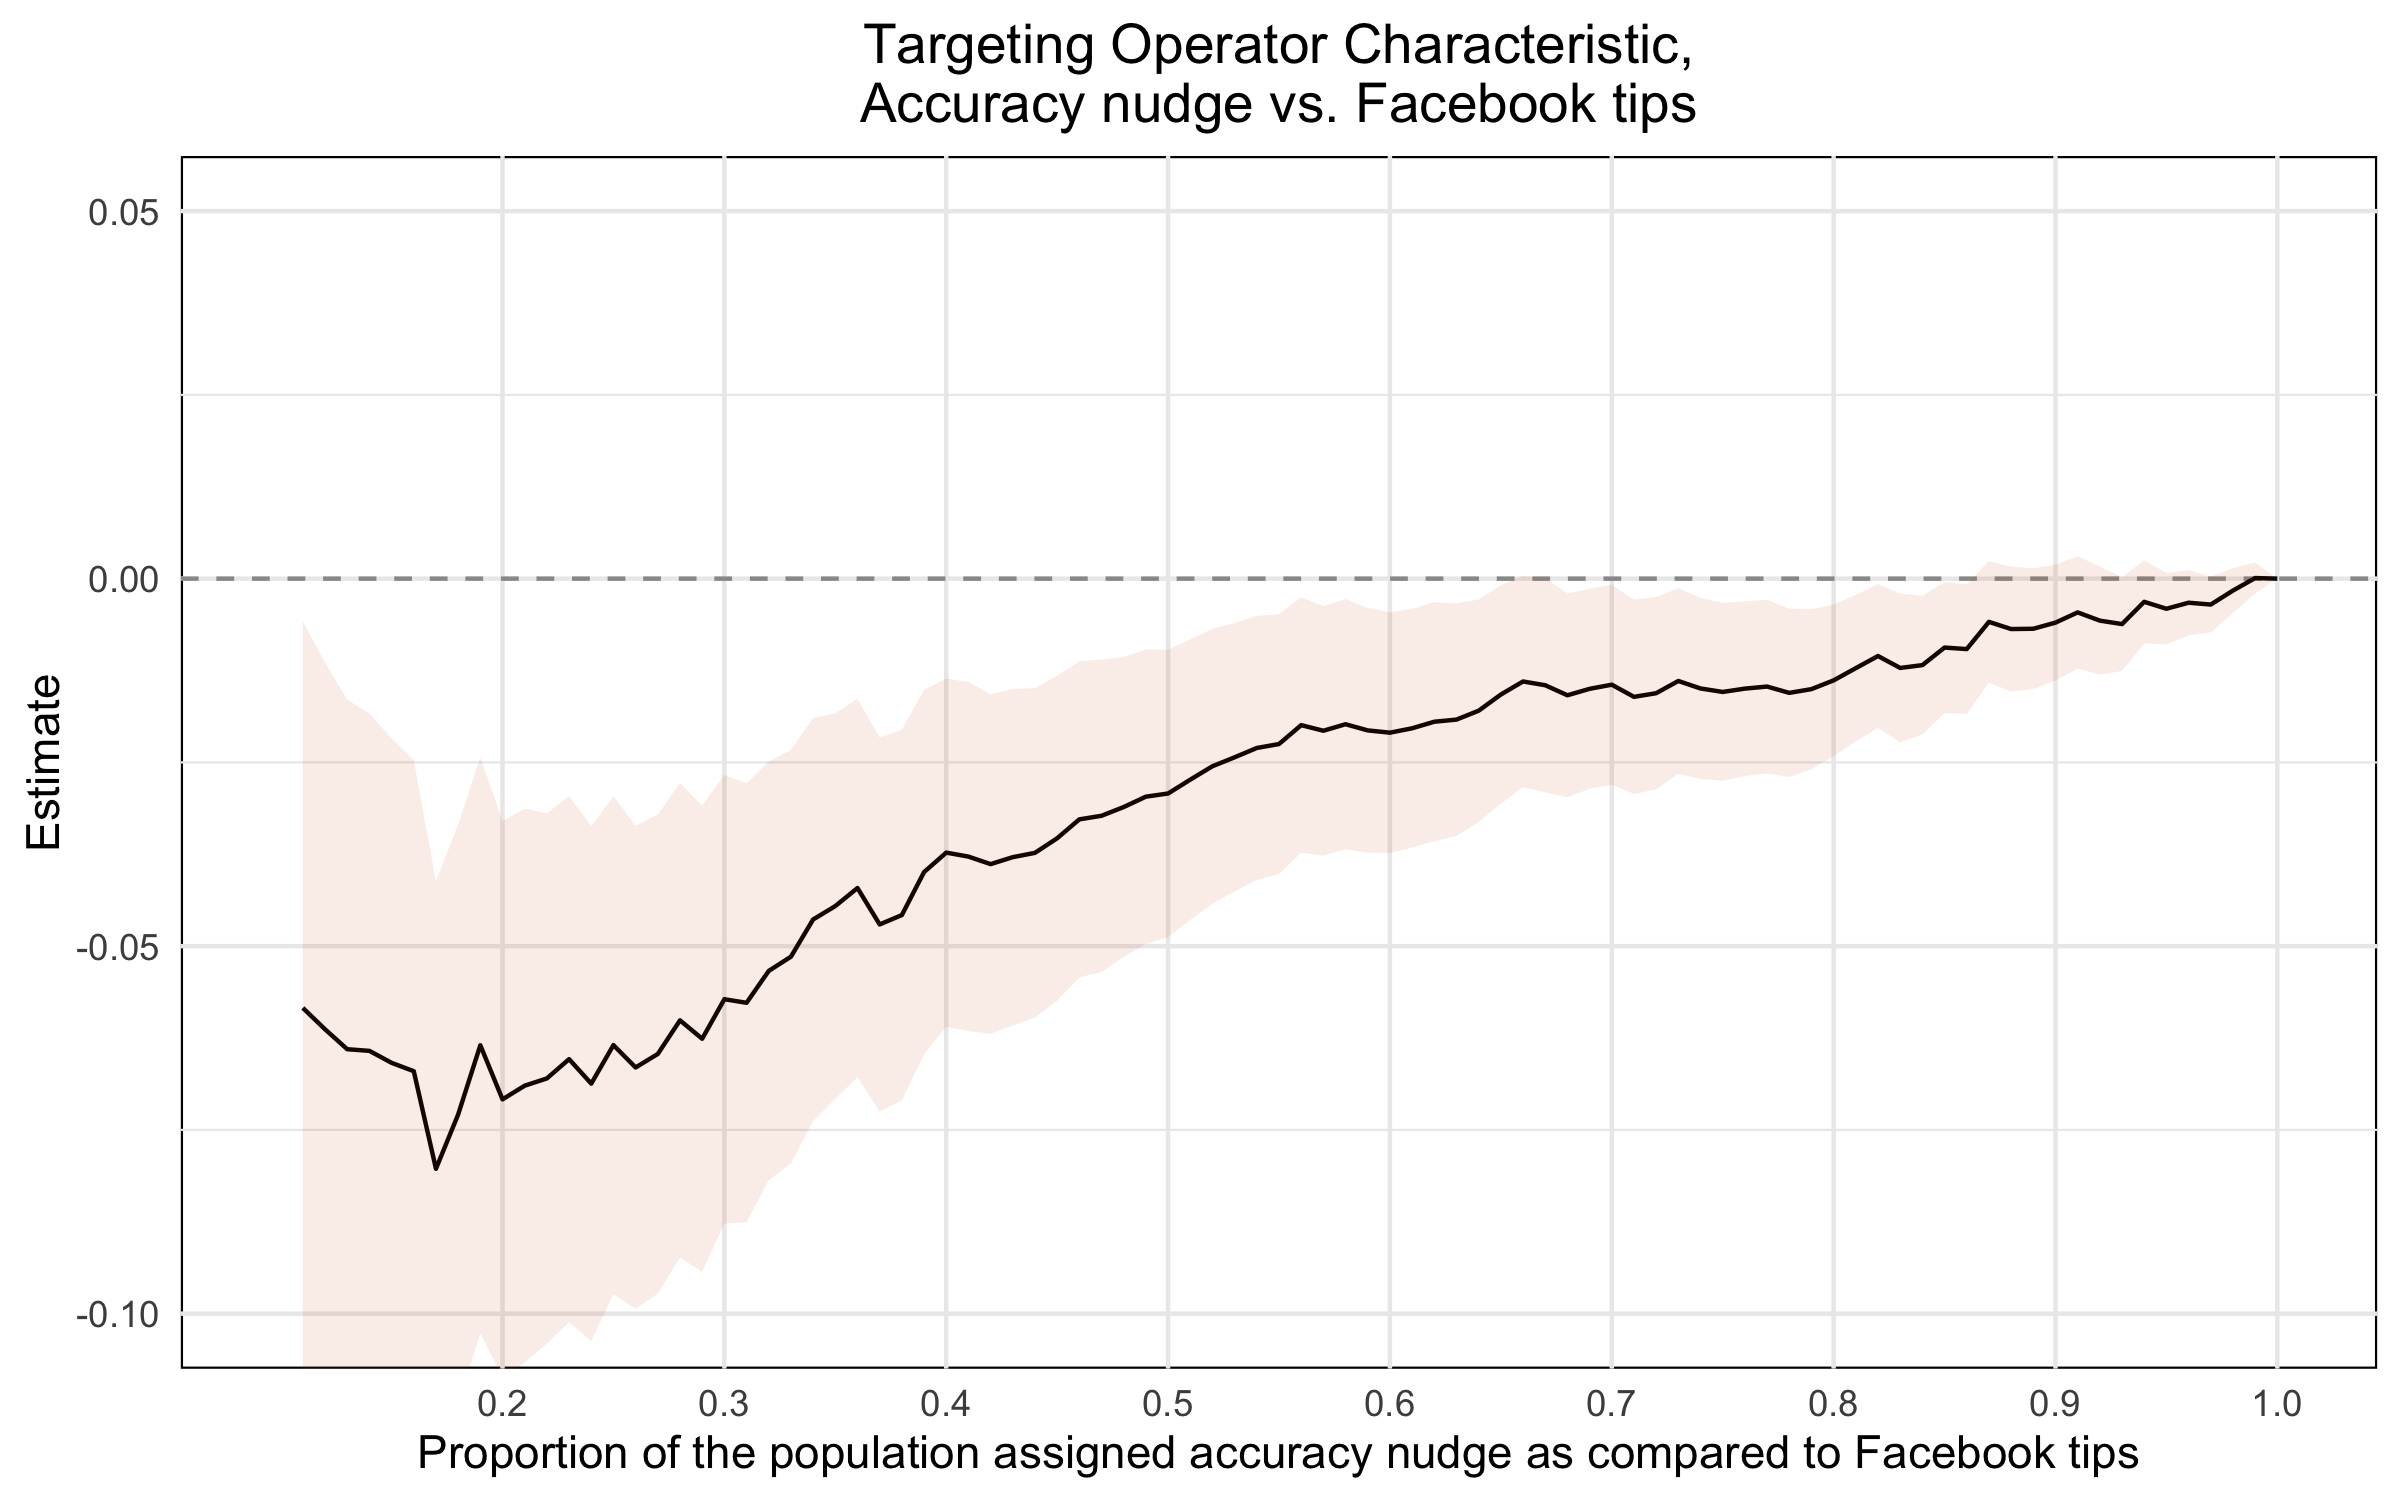
\includegraphics[width=\textwidth]{../analysis/figures/rate_accuracy_vs_facebook.png} 
   \caption{\textbf{Targeting operator characteristic curve, comparing the accuracy nudge and Facebook tips.} The outcome measure is the difference in proportion of false stimuli participants reported wanting to share, either as a Facebook post or privately in Facebook Messenger, between the accuracy nudge and Facebook tips. The y-axis represents differences in this measure if the users receiving the accuracy nudge were assigned according to a prioritization rule, as compared to at random. The shaded region shows the 95\% confidence interval.}
   \label{fig:RATE}
\end{figure}

To evaluate the overall effect of targeting, we consider the causal forest model learned for prioritization rule above as a contextual policy: if the predicted difference between the accuracy nudge and the Facebook tips treatment is negative (indicating that the accuracy nudge is more effective at decreasing false sharing), our policy assigns the accuracy nudge; otherwise the Facebook tips treatment is assigned. Again, as the policy is learned on the learning data and evaluated on the evaluation data, we avoid concerns with over-fitting.  

When the model is applied to the evaluation data, our optimal contextual policy assigns 43.5\% of participants to Facebook tips, which is the best uniform policy for decreasing sharing of false stimuli. Optimally assigning these treatments, we achieve a treatment effect of -3.9 percentage points (SE = 1.1) in decreasing false sharing intentions.  We saw in Table~\ref{tab:main_results} that we achieve larger magnitude treatment effects in decreasing false sharing intentions through our contextual policy as compared to either the accuracy nudge or the Facebook tips treatments assigned uniformly (differences of -2.0 pp, SE = 0.8 and -0.8 pp, SE = 0.8, one-sided p-values of 0.009 and 0.150, respectively). %next round add 1 sentence interpretation/conclusion here...

In Table~\ref{tab:heterogeneity_best}, we see that our contextual policy learned on the learning data is appropriately assigning participants to the respective respondent-level conditions: participants for whom assignment under the learned optimal policy is Facebook tips on average intend to share false information at lower rates under the Facebook tips treatment as compared to the accuracy nudge (difference of 3.8, SE = 1.4); the reverse is true directionally for the participants assigned the accuracy nudge under the learned optimal policy (difference of -1.6, SE = 1.5).  


\begin{table}[H]
\small
   \centering
\resizebox{\textwidth}{!}{ 
\begin{tabular}{lccccccc}
&    & \multicolumn{3}{c}{\textbf{False}} & \multicolumn{3}{c}{\textbf{True}} \\
& \textbf{Combined}& Any sharing & Messenger & Timeline & Any sharing & Messenger & Timeline \\
 \cmidrule(lr){2-2}  \cmidrule(lr){3-5}  \cmidrule(lr){6-8}
\multicolumn{4}{l}{\textbf{Optimal assignment == Accuracy nudge} (n = 4,967)} \rule{0pt}{1.2\normalbaselineskip} \\
\hspace{1em} Accuracy & \num{-0.162} & \num{0.396} & \num{0.349} & \num{0.341} & \num{0.681} & \num{0.588} & \num{0.637}\\
& (\num{0.031}) & (\num{0.010}) & (\num{0.009}) & (\num{0.009}) & (\num{0.010}) & (\num{0.010}) & (\num{0.010})\\
\hspace{1em} Facebook tips & \num{-0.220} & \num{0.412} & \num{0.363} & \num{0.352} & \num{0.687} & \num{0.602} & \num{0.639}\\
 & (\num{0.038}) & (\num{0.012}) & (\num{0.012}) & (\num{0.011}) & (\num{0.013}) & (\num{0.013}) & (\num{0.013})\\
   \cmidrule(lr){2-8}
 \hspace{1em} Difference & \num{0.058} & \num{-0.016} & \num{-0.014} & \num{-0.012} & \num{-0.006} & \num{-0.014} & \num{-0.001}\\
  & (\num{0.050}) & (\num{0.015}) & (\num{0.015}) & (\num{0.015}) & (\num{0.016}) & (\num{0.016}) & (\num{0.016})\\
\multicolumn{4}{l}{\textbf{Optimal assignment == Facebook tips} (n = 5,716)} \rule{0pt}{1.2\normalbaselineskip} \\
\hspace{1em} Accuracy & \num{-0.478} & \num{0.445} & \num{0.401} & \num{0.345} & \num{0.622} & \num{0.547} & \num{0.534}\\
 & (\num{0.027})  & (\num{0.009}) & (\num{0.009}) & (\num{0.009}) & (\num{0.009}) & (\num{0.009}) & (\num{0.009})\\
\hspace{1em} Facebook tips & \num{-0.453}& \num{0.407} & \num{0.367} & \num{0.330} & \num{0.589} & \num{0.516} & \num{0.513}\\
 & (\num{0.035}) & (\num{0.011}) & (\num{0.011}) & (\num{0.011}) & (\num{0.011}) & (\num{0.011}) & (\num{0.011})\\
   \cmidrule(lr){2-8}
 \hspace{1em} Difference & \num{-0.025}& \num{0.038}** & \num{0.034}* & \num{0.014} & \num{0.033}* & \num{0.031}* & \num{0.021}\\
  & (\num{0.044})& (\num{0.014}) & (\num{0.014}) & (\num{0.014}) & (\num{0.015}) & (\num{0.015}) & (\num{0.015})\\
\hline
\multicolumn{4}{l}{\textbf{Grand difference}} \rule{0pt}{1.2\normalbaselineskip} \\
& \num{0.083}&   \num{0.054}* & \num{0.048}* & \num{0.026} & \num{0.039}+ & \num{0.045}* & \num{0.023}\\
  & (\num{0.066}) & (\num{0.021}) & (\num{0.021}) & (\num{0.020}) & (\num{0.022}) & (\num{0.022}) & (\num{0.021})\\
   \end{tabular}
   }
   \caption{\textbf{Response under counterfactual uniform respondent treatment conditions, by contextual policy assignment.} Estimates are of mean response under the two respondent-level treatments. Estimates are produced from an augmented inverse probability weighted estimator, as described in Section~\ref{section:estimation}, within specified subgroups. For contrasts only, under two-sided hypothesis tests: \textsuperscript{+} $p<0.1$, \textsuperscript{*} $p < 0.05$, \textsuperscript{**} $p < 0.01$, \textsuperscript{***} $p < 0.001$.}
   \label{tab:heterogeneity_best}
\end{table}


Previous research has raised the question of %been able to determine %% want to be careful bc not necessarily tried...?
whether Facebook tips and an accuracy nudge both operate along the mechanism of increasing attention to accuracy,  as suggested for the accuracy nudge by \cite{pennycook_epstein_mosleh_arechar_eckles_rand_2019}, 
or rather whether the Facebook tips improve ability to evaluate stimuli, as proposed by \cite{guessetal2020digital}. The heterogeneity we find in treatment effects between the two groups (difference of 3.8 pp, SE = 1.4) suggests, however, that there are differences in how users respond to these treatments, and different types of people respond differently to each treatnent. 

To better understand differences in the types of people that are most responsive to each of these interventions, we compare differences across our selected covariates. 
The 46.5\% of participants assigned to the accuracy nudge % can we say: "for whom accuracy is optimal" ?
are, on average, more digitally literate, more likely to have more scientific knowledge,
more likely to be male, older, and directionally more likely to be aligned with the governing political party than those assigned to the Facebook tips treatment (see Figure~\ref{fig:heterogeneity_covariates}).

% LR ADD TO NEXT DRAFT: MAKE bigger deal of this - given the numerous (at least 3) studies that say accuracy nudges work/scale... depending on how large these groups are in the population of interest (and if results operate same way in other contexts...) might not be effective. Main takeaway: accuracy nudge does not work for everyone.

\begin{figure}[H] %  figure placement: here, top, bottom, or page
   \centering
   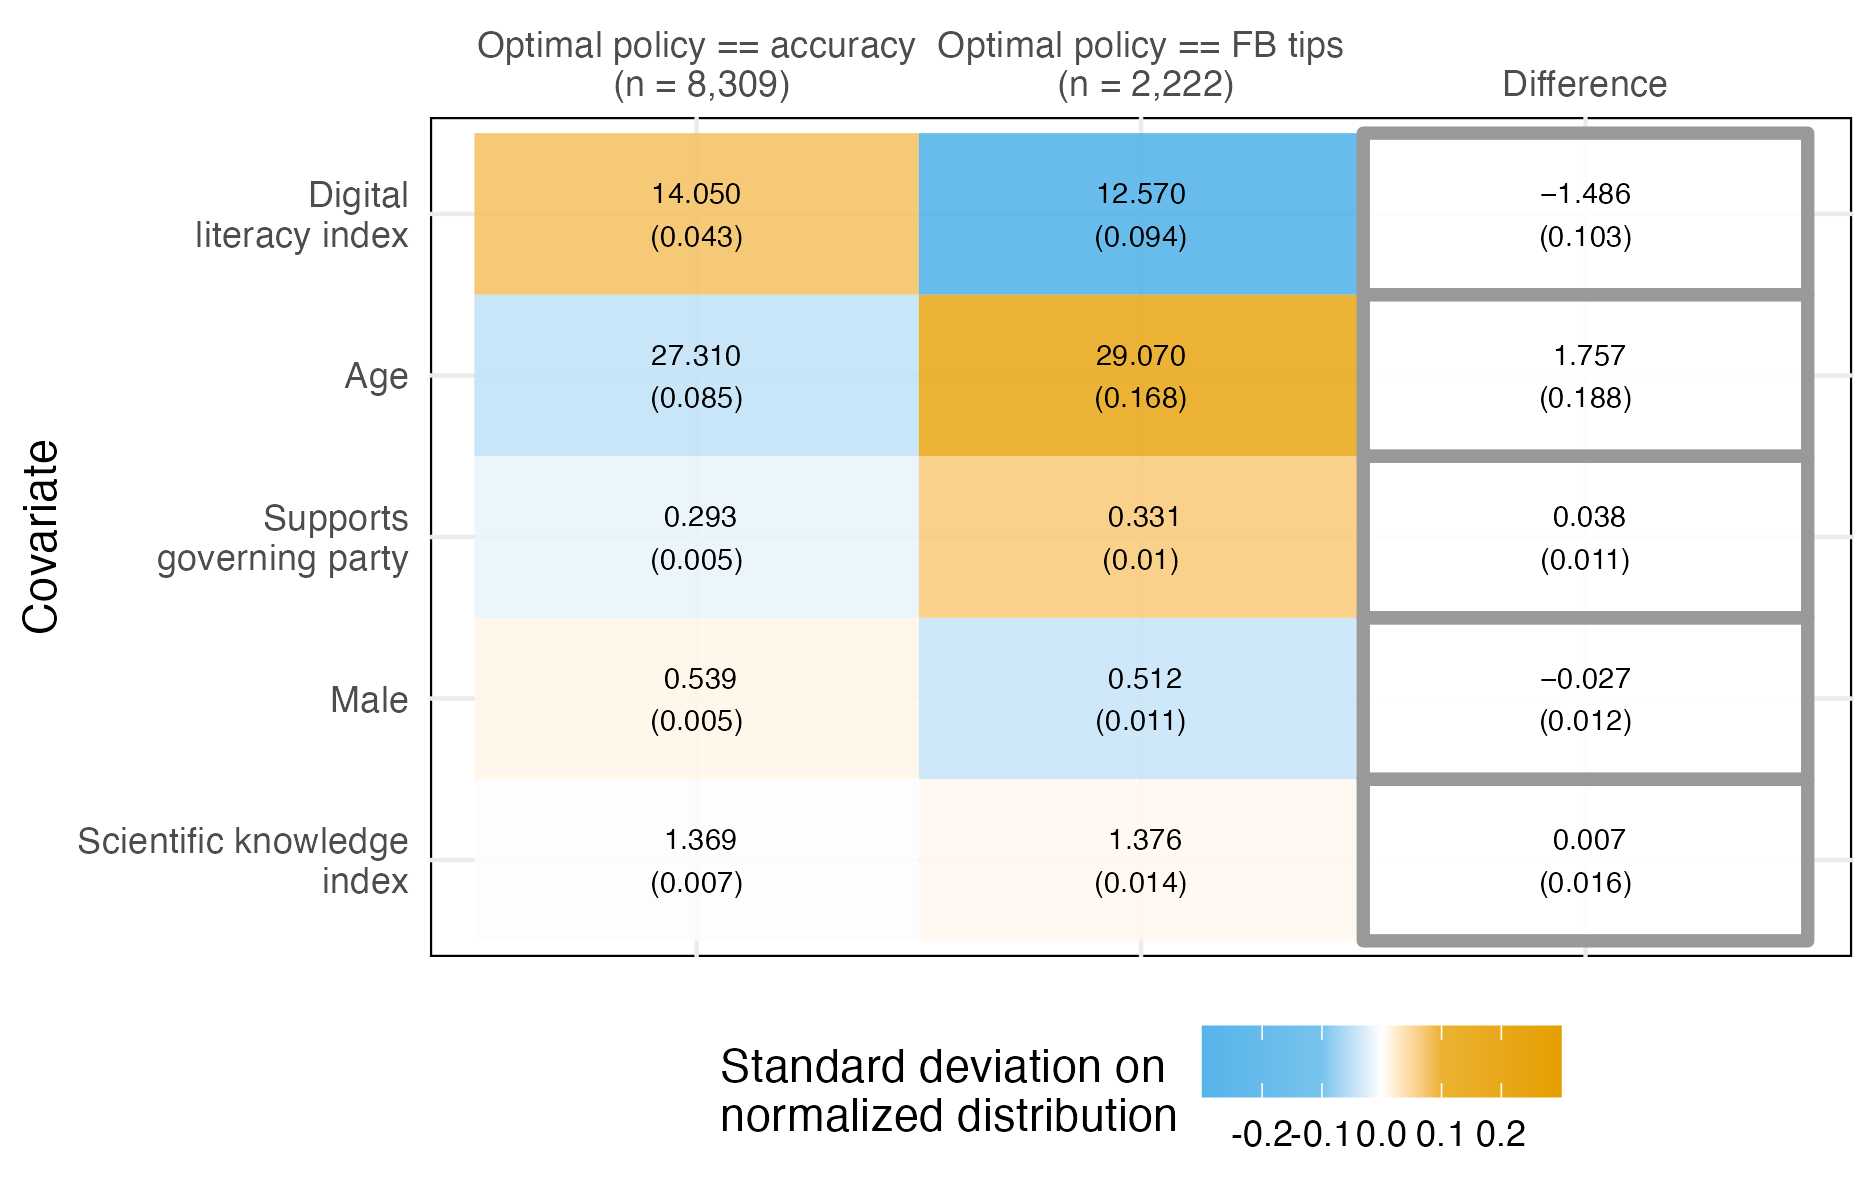
\includegraphics[width=\textwidth]{../analysis/figures/covariate_optimal.png} 
   \caption{\textbf{Selected covariate means between participants assigned to the accuracy nudge as compared to participants assigned to Facebook tips under the contextual policy.} Covariates are ordered by size of standardized deviation between the two groups. }
   \label{fig:heterogeneity_covariates}
\end{figure}


\paragraph{Sharing channel}
Overall, the Facebook tips treatment has directionally larger effects on mitigating false sharing intentions relative to the accuracy nudge (difference of -1.3 pp, SE = 0.9), but it also directionally reduces true sharing intentions (difference of -1.5 pp, SE = 1.0); this results in the accuracy nudge scoring better on our combined response measure (difference of -0.014, SE = 0.03). To further investigate variations in how these two treatments operate, we consider the secondary dimension of our response measurement, sharing channel. 

The Facebook tips treatment and the accuracy nudge are both effective at moving false sharing intentions on the timeline (-3.0 pp, SE = 1.0; -2.6 pp, SE = 0.9 respectively)  and on Messenger (-2.9 pp, SE = 1.1; -1.8 pp, SE = 1.0 respectively)  relative to control. % Discuss as proportion? As the rates of false sharing on timeline under control are lower relative to Messenger... 
The Facebook tips treatment is directionally relatively more effective at also reducing false sharing intentions on Messenger (difference of -0.9, SE = 1.0). 

This difference in effects by channel may speak to the mechanisms by which these two treatments work. We may suppose that one reason that respondents share false stimuli at all is that they are not able to discern between true and false stimuli. As noted, we do see evidence of discernment under control, where respondents share false stimuli less on both channels relative to true stimuli. If treatments help users learn how to discern false stimuli from true stimuli, as is the objective of the Facebook tips treatment, we should see effects both on timeline and on Messenger for false sharing intentions. We would also predict that these effects would be relatively larger for respondents who are less able to differentiate false from true stimuli under control, as we discuss in the next section. 

However, if sharing of false stimuli were merely due to users misattributing truth to some proportion of false stimuli, all else equal, under control we should expect that sharing rates by channel for false stimuli would be proportional to those for true stimuli. Rather, we see variation in users' preferred channel for sharing between true and false stimuli under control. An alternative mechanism through which treatment affects outcomes might be that the treatments are shifting attention to the accuracy of stimuli, as has been proposed for the accuracy nudge. For users who are already able to discern between true and false stimuli, it is ambiguous how this should inform relative effects on the channel by which respondents share false stimuli. It may be that users are wary of sharing false posts publicly on their timeline out of fear for reputational costs they would incur from peers if they were caught sharing misinformation \citep{altay2022so}, but they may still believe that the posts may be of interest or value to share with individual contacts. If increased attention to the accuracy highlights concerns about reputational costs of publicly sharing false stimuli, this would result in larger relative effects on timeline as compared to Messenger false sharing intentions, as we see under the accuracy nudge.  % indicating even when ppl say they want to share false posts, they may have some indication/hesitancy about sharing it publicly - want to share privately to individual - perhaps over fear of ridicule/concerns that is may be false…


\paragraph{Heterogeneous response and treatment effects}

We find that users with low digital literacy, participants aligned with the ruling party,  participants with low scientific knowledge, and younger participants intend to share more false stimuli. For these ``worst offenders'' we find that assigning the respondent-level treatments on average decreases false sharing as compared to control among participants with low digital literacy (-4.3, SE = 1.4), men (-3.3, SE = 1.3), and participants with low scientific knowledge (-4.5, SE =1.3). (See Table~\ref{tab:heterogeneity_treatment}.) The pooled respondent-level interventions do not reduce sharing of false posts among younger participants but do among older ones. Similarly, there is no effect of the pooled respondent treatments on false sharing among those aligned with the political party in power, but we do see a significant effect among those not aligned. However, \textit{differences} in treatment effects across groups are for the most part only statistically significant when comparing users with low to those with high levels of scientific knowledge.

This may reflect, as other studies have documented, that affective partisanship and motivated reasoning influence sharing of misinformation \citep{sanchez2021cognitive}. It is somewhat surprising, however, that even for less (blatantly) political information of COVID-19 best practices, these interventions are unable to move ruling party supporters. 
%Young people and ruling party supporters may be large shares of the social media populations in these countries and elsewhere. Hence, it is important to recognize that these interventions may not be effective for these subgroups. Further research is required to understand what is effective at reducing their intentions to share false information, but this study critically finds that these interventions are not universally effective. 

The largest treatment effects on false sharing intentions were for users with below median digital literacy and below median scientific knowledge. For these users, like users on average, the Facebook tips treatment was more effective than the accuracy nudge (difference of 1.0 pp, SE = 1.3 for digital literacy; 1.4 pp, SE = 1.3 for scientific knowledge) (see Tables~\ref{tab:heterogeneity_treatment_facebook} and~\ref{tab:heterogeneity_treatment_accuracy} in the SI). One possible explanation is that lower digital literacy and lower scientific knowledge users may be less able to differentiate false from true stimuli, and so the larger effects on these groups would be consistent with these users learning how to better evaluate stimuli under the Facebook tips treatment. In other words, the first order concern for these users is to equip them with the techniques and skills to identify misinformation, whereas for others with higher levels of digital skills and scientific knowledge interventions reminding users to focus on accuracy are more effective. 

For users with below median digital literacy and below median scientific knowledge, treatment effects under Facebook tips were driven by relatively larger effects on private sharing on Messenger as compared to public sharing on their timelines (difference of 1.1 pp, SE = 1.2 for digital literacy; 0.9 pp, SE = 1.1 for scientific knowledge), whereas for the accuracy nudge, effects on timeline as compared to messenger sharing are comparable for these groups (difference of -0.3 pp, SE = 1.1 for digital literacy; 0.1 pp, SE = 1.1 for scientific knowledge). The overall larger effects on private Messenger sharing for Facebook tips as compared to the accuracy nudge is concentrated among these users. This may suggest that the Facebook tips treatment not only helps users to better differentiate between true and false stimuli, but for some types of users, it also makes them less likely to privately share stimuli that they already know is false.



% In particular, if we think that sharing false posts on timeline is particularly problematic - because it has the greatest potential reach - then interventions should target those aligned with the ruling party, users with below median digital literacy, and men.
% And aligned partisans are sharing the most false posts on timeline (out of all subgroups) *bc they share the most in general (across all types of posts/channels)


\begin{table}[H]
\small
   \centering
\resizebox{\textwidth}{!}{ 
\begin{tabular}{lccccccc}
&    & \multicolumn{3}{c}{\textbf{False}} & \multicolumn{3}{c}{\textbf{True}} \\
& \textbf{Combined}& Any sharing & Messenger & Timeline & Any sharing & Messenger & Timeline \\
 \cmidrule(lr){2-2}  \cmidrule(lr){3-5}  \cmidrule(lr){6-8}
\multicolumn{4}{l}{\textbf{Age}} \rule{0pt}{1.2\normalbaselineskip} \\
\hspace{1em} Below median  	& \num{0.002} & \num{-0.019} & \num{-0.021} & \num{-0.017} & \num{-0.026}+ & \num{-0.020} & \num{-0.034}*\\
\hspace{1.5em} (n = 5,412)	& (\num{0.039}) & (\num{0.013}) & (\num{0.013}) & (\num{0.012}) & (\num{0.014}) & (\num{0.014}) & (\num{0.014})\\
\hspace{1em} Above median  	& \num{0.104}* & \num{-0.032}* & \num{-0.030}* & \num{-0.035}** & \num{0.009} & \num{0.020} & \num{0.003}\\
 \hspace{1.5em} (n = 5,271) 	& (\num{0.045}) & (\num{0.014}) & (\num{0.013}) & (\num{0.013}) & (\num{0.013}) & (\num{0.014}) & (\num{0.014})\\
\cmidrule(lr){2-8}
 \hspace{1em} Difference 		& \num{-0.102}+ & \num{0.013} & \num{0.009} & \num{0.019} & \num{-0.035}+ & \num{-0.040}* & \num{-0.037}+\\
 						& (\num{0.060}) & (\num{0.019}) & (\num{0.018}) & (\num{0.018}) & (\num{0.019}) & (\num{0.020}) & (\num{0.019})\\
  \multicolumn{4}{l}{\textbf{Gender}}  \rule{0pt}{1.2\normalbaselineskip}\\
\hspace{1em}Not male		& \num{0.038} & \num{-0.020} & \num{-0.024}+ & \num{-0.020} & \num{-0.025}+ & \num{-0.003} & \num{-0.030}*\\
\hspace{1.5em} (n = 5,050) 	& (\num{0.042}) & (\num{0.014}) & (\num{0.013}) & (\num{0.012}) & (\num{0.014}) & (\num{0.014}) & (\num{0.014})\\
\hspace{1em} Male  			& \num{0.066} & \num{-0.030}* & \num{-0.026}* & \num{-0.031}* & \num{0.006} & \num{0.003} & \num{-0.004}\\
\hspace{1.5em}  (n = 5,633)	& (\num{0.042}) & (\num{0.013}) & (\num{0.013}) & (\num{0.013}) & (\num{0.013}) & (\num{0.013}) & (\num{0.013})\\
 \cmidrule(lr){2-8}
 \hspace{1em} Difference 			& \num{-0.029} & \num{0.011} & \num{0.003} & \num{0.011} & \num{-0.031} & \num{-0.007} & \num{-0.026}\\
 \hspace{1.5em} 				& (\num{0.059}) & (\num{0.019}) & (\num{0.018}) & (\num{0.018}) & (\num{0.019}) & (\num{0.020}) & (\num{0.019})\\  
 \multicolumn{4}{l}{\textbf{Political allegiance}} \rule{0pt}{1.2\normalbaselineskip}\\
\hspace{1em} Not aligned  		& \num{0.095}** & \num{-0.034}** & \num{-0.030}** & \num{-0.039}*** & \num{-0.008} & \num{0.003} & \num{-0.014}\\
\hspace{1.5em} (n = 7,570) 		& (\num{0.035}) & (\num{0.011}) & (\num{0.011}) & (\num{0.011}) & (\num{0.011}) & (\num{0.012}) & (\num{0.012})\\
\hspace{1em} Aligned  			& \num{-0.049} & \num{-0.005} & \num{-0.013} & \num{0.005} & \num{-0.011} & \num{-0.008} & \num{-0.022}\\
\hspace{1.5em} (n = 3,113)		& (\num{0.055}) & (\num{0.018}) & (\num{0.017}) & (\num{0.017}) & (\num{0.017}) & (\num{0.018}) & (\num{0.017})\\
  \cmidrule(lr){2-8}
 \hspace{1em} Difference 			& \num{0.144}* & \num{-0.029} & \num{-0.017} & \num{-0.044}* & \num{0.004} & \num{0.011} & \num{0.008}\\
\hspace{1.5em} 				& (\num{0.065}) & (\num{0.021}) & (\num{0.020}) & (\num{0.020}) & (\num{0.021}) & (\num{0.021}) & (\num{0.021})\\
 \multicolumn{4}{l}{\textbf{Digital literacy index }}  \rule{0pt}{1.2\normalbaselineskip}\\
\hspace{1em} Below median 		& \num{0.056} & \num{-0.041}** & \num{-0.039}** & \num{-0.035}** & \num{-0.025}+ & \num{-0.010} & \num{-0.026}*\\
\hspace{1.5em}  (n = 5,443)		& (\num{0.042}) & (\num{0.013}) & (\num{0.013}) & (\num{0.013}) & (\num{0.013}) & (\num{0.013}) & (\num{0.013})\\
\hspace{1em} Above median 		& \num{0.049} & \num{-0.009} & \num{-0.011} & \num{-0.016} & \num{0.008} & \num{0.011} & \num{-0.005}\\
\hspace{1.5em} (n = 5,240)  		& (\num{0.042}) & (\num{0.014}) & (\num{0.013}) & (\num{0.012}) & (\num{0.014}) & (\num{0.014}) & (\num{0.014})\\
 \cmidrule(lr){2-8}
\hspace{1em} Difference 			& \num{0.007} & \num{-0.033}+ & \num{-0.028} & \num{-0.019} & \num{-0.033}+ & \num{-0.021} & \num{-0.021}\\
 							& (\num{0.060}) & (\num{0.019}) & (\num{0.018}) & (\num{0.018}) & (\num{0.019}) & (\num{0.020}) & (\num{0.019})\\
 \multicolumn{4}{l}{\textbf{Scientific knowledge index }}  \rule{0pt}{1.2\normalbaselineskip}\\
\hspace{1em}   Below median  			& \num{0.094}* & \num{-0.043}** & \num{-0.047}*** & \num{-0.042}*** & \num{-0.027}* & \num{-0.012} & \num{-0.033}*\\
\hspace{1.5em} (n = 5,677)			& (\num{0.040}) & (\num{0.013}) & (\num{0.013}) & (\num{0.012}) & (\num{0.013}) & (\num{0.014}) & (\num{0.013})\\
\hspace{1em}   Above median			& \num{0.006} & \num{-0.006} & \num{-0.001} & \num{-0.008} & \num{0.012} & \num{0.014} & \num{0.004}\\
\hspace{1.5em}  (n = 5,006) 			& (\num{0.044}) & (\num{0.014}) & (\num{0.013}) & (\num{0.013}) & (\num{0.014}) & (\num{0.014}) & (\num{0.014})\\
 \cmidrule(lr){2-8}
\hspace{1em}   Difference 			& \num{0.087} 	& \num{-0.037}+ & \num{-0.045}* & \num{-0.034}+ & \num{-0.039}* & \num{-0.026} & \num{-0.037}+\\
 								& (\num{0.060}) & (\num{0.019}) & (\num{0.018}) & (\num{0.018}) & (\num{0.019}) & (\num{0.020}) & (\num{0.019})\\
    \end{tabular}
   }
   \caption{\textbf{Heterogeneity in treatment effects under averaged respondent-level treatments by selected covariates.} Estimates are of treatment effects averaged across the two respondent-level treatments, in contrast with the control condition. Estimates are produced from an augmented inverse probability weighted estimator, as described in Section~\ref{section:estimation}, within specified subgroups. Under two-sided hypothesis tests: \textsuperscript{+} $p<0.1$, \textsuperscript{*} $p < 0.05$, \textsuperscript{**} $p < 0.01$, \textsuperscript{***} $p < 0.001$.}
  \label{tab:heterogeneity_treatment}
\end{table}

%\begin{figure}[H]
%\includegraphics[width = \textwidth]{../analysis/figures/any_sharing_by_covariates_te_comparisons_false.png}
%\caption{Response under the control condition. The outcome measure is the proportion of true or false stimuli participants reported wanting to share, either as a Facebook post or privately in Facebook Messenger. Estimates are produced from an augmented inverse probability weighted estimator, as described in Section~\ref{section:estimation}, within specified subgroups.}
%\label{fig:treatments}
%\end{figure}\todo{Alternative figure}



%\begin{figure}[H]
%\centering
%\includegraphics[width = \textwidth]{../analysis/figures/r_accuracy_scores_any_false_r_tips_facebook_scores_any_false_optimal_assignment.png}
%   \caption{\textbf{Response under counterfactual uniform respondent treatment conditions, by contextual policy assignment.} Estimates are produced from an augmented inverse probability weighted estimator, as described in Section~\ref{section:estimation}, within specified subgroups.}
%   \label{fig:heterogeneity_best}
%\end{figure}



%%%%%%%%%%%%%%%%%%%%%%%%%%%%%%%%%%%%%%%%%%%%
%DISCUSSION
%%%%%%%%%%%%%%%%%%%%%%%%%%%%%%%%%%%%%%%%%%%%


\section{Discussion}

We find both the accuracy nudge and Facebook tips are effective at curbing intentions to share misinformation. These treatments relate to two theories about why people are susceptible to misinformation.%
\footnote{
 There are of course additional theories to explain why people are susceptible to or share misinformation---for instance for identity-based or ideological reasons \citep{nyhan2010corrections}, or because something is funny or interesting if true \citep{altay2022if}. %These theories are not the focus of this study, however, and although we did ask about partisanship we do not see substantive differences in treatment effects by party ID.% 
}
The first from cognitive science suggests that people consume social media content quickly, react intuitively and do not stop to think about whether something is true or false. This reasoning suggests that people need to be reminded or ``nudged'' to consider the accuracy of posts, otherwise it may not be something they consider before sharing a post \citep{pennycook2021psychology, pennycook2021shifting}. A second rationale suggests that people simply do not know how to identify misinformation or lack the information to be able to do so \citep{ecker2022psychological}. This \textit{information deficit model} prescribes providing training or tips to equip individuals to be able to spot misinformation in their news feed. Importantly, these are not mutually exclusive theories and people may suffer from both challenges---but whether one intervention is more successful, on average, than the other is important to understand as well as for which types of people one prescription may be better than the other. 

Other studies have found similar positive effects of accuracy prompts, including among quota-matched samples in 16 countries \citep{arechar2022understanding} and in a meta-analysis of 20 accuracy experiments with a total sample size over 20,000 \citep{pennycook2022accuracy}. Facebook tips have also been shown to effectively reduce belief in false headlines in the US and India \citep{guessetal2020digital}, indicating that both treatments may be scalable solutions for the global misinformation challenge. \citet{pennycook2021shifting} provide evidence that increased attention to the accuracy of articles is the mechanism driving the efficacy of the accuracy nudge. 

We also evaluated two headline-level treatments. We tested a factcheck intervention that has been used by several platforms and adds ``disputed'' flags to false posts. We also tested the related articles intervention that Facebook has used in the past---providing links to related articles under misleading or false posts \citep{ghosh2017facebook}.

Warning labels on posts have been found to be effective at helping users identify misinformation \citep{clayton2020real} and reduce individual's willingness to share fake-news headlines \citep{mena2020cleaning} in the context of political information in respondent samples from the Global North.  For COVID-19 information, \citet{kreps2020medical} find the effectiveness of these tags to depend on context, specifically that they worked for only one out of three false COVID headlines tested. Recent evidence suggests fact checks can improve discernment (belief) among samples from Africa, Latin America, and the UK \citep{porter2021global}. \citet{brashier2021timing} also find that the timing of fact checking matters---specifically that debunking misinformation after the headline is shown was more successful than contemporaneous tags, but do not test how these flags and warnings affect sharing behavior. 


\textcolor{red}{ % REFRAME IN CONTEXT OF FINDINGS, discuss what means for future work
Interventions that flag specific posts rely on resource intensive fact-checking sources to verify the veracity of individual posts before applying such labels.  Most posts are only flagged after they have circulated online and become popular, having the opportunity to inflict damage before factchecks and labels can be applied. A strategy of fact-checking and adding labels requires keeping up with new misinformation being generated. General interventions delivered to users while they are on a particular platform, on the other hand, are less resource intensive, can be applied at any time, and are much more easily delivered en masse. \todo{cut? or move to discussion? or make 1 sentence in prior par?}\todo{whether we include here/intro depends on how much of contribution we see this as - I see it mostly as a nice point to make: we were able to evaluate on same sample/time/measures a ton of treatment across these 2 types - we see respondent-level more effective --> might be worth investing more in finding successes of these types (bc cheaper + easier to scale). so I (LR) might propose moving this par to discussion...}
}

\todo{Moved the above here in case we want to use.}

This study, like others of its kind, has limitations. Importantly, the data come from a survey experiment, rather than a field experiment. However, the design of the study offers enhanced realism for participants beyond the standard approach of recruitment of samples through survey firms, and implementation of surveys on web browser-based platforms. Instead, we recruit social media users on the Facebook platform itself, where they would normally come into contact with online (mis)information about COVID-19. We keep participants on the platform interacting with a Messenger bot, which may feel somewhat more naturalistic than answering survey questions using another software, but is still an experimenter-controlled environment. This control facilitated more straightforward measurement, and also reduces ethical concerns about the possibility of the experiment facilitating the spread of COVID misinformation during a global pandemic. 

Acknowledging these limitations, we believe this study offers insights useful for fighting online misinformation globally. The key insight is that low-cost and scalable accuracy nudges and tips for spotting misinformation delivered to users as they scroll social media can be effective in many diverse contexts. This study provides evidence that such interventions are more effective than many others often tested by academics and used by platforms. Platforms may be more likely to deliver such interventions knowing that they help reduce sharing of misinformation without harming sharing of true information. Policymakers and platforms may also consider targeting interventions to those prone to share misinformation and not waste resources or risk a worse user experience by \textit{not} directing such interventions to groups for whom they are ineffective. Overall, these policies delivered to participants are much more cost effective than headline-specific interventions that require time and effort from human or AI fact checkers.

%Ours is one of only a few studies examining Facebook's related articles policy \citep[see also][]{bode2015related}, hence more research is needed. The fact that we do not see effects from fact-checking interventions in this setting should raise questions given the existing evidence of disputed labels and warnings from the US and other high-income countries. However, we believe that these results may vary across settings given the variations in context, specifically the general levels of digital literacy and abilities to discern fact from fiction. For instance, when we analyze the headline-level interventions by baseline-levels of sharing ``discernment'' (pre-treatment sharing of true $>$ false information), we find that there is a group of more discerning participants for whom showing related articles under false posts reduces false sharing compared to control. %\todo{add figure/table in SI}
%
%Specifically, participants with pretreatment sharing discernment above the sample median share false news less under related articles treatment as compared to control ($p < 0.05$), participants below median share false news more under related articles ($p < 0.06$), and the difference is significant at $p < 0.01$. Participants with above median baseline levels of sharing discernment share false stimuli (along either channel) 19.1 percent of the time. Under the related articles treatment, this sharing is decreased by 1.4 pp, a 7.2 percent reduction. These findings perhaps hint at the idea that more ambiguous post-level interventions such as showing related articles are only effective among already well-discerning individuals. This may also help to explain our general finding of no effects from headline-level treatments among our sample---who may have lower baseline discernment than samples from high-income countries that may have generally higher levels of education or have greater digital literacy. More research with samples outside of the Global North is required to understand which interventions are effective and why some treatments that work in certain settings are not effective in others.

\todo{Add more about what we can say re. differences in FB tips and accuracy}

\paragraph{Experimenter demand effects}
To attempt to reduce experimenter demand effects, we embedded treatments in a longer survey block about general social media usage. If users' post-treatment responses were, however, based on perceptions of what researchers want, we might expect high digital literacy users to be the most savvy to the survey objectives, and treatment effects to be largest for this group. Instead, we see the reverse is true. The variation in treatment effects by channel also provides evidence against experimenter demand effects: if users were only responding to perceived experimenter objectives, we might expect effects to be uniform across channels. 


%%%%%%%%%%%%%%%%%%%%%%%%%%%%%%%%%%%%%%%%%%%%
%MATERIALS AND METHODS
%%%%%%%%%%%%%%%%%%%%%%%%%%%%%%%%%%%%%%%%%%%%

\section{Methods}

\subsection{Data and recruitment}\label{section:data}
Our sample is recruited from Facebook users in Kenya and Nigeria. Kenya and Nigeria represent two of Facebook's top three largest user bashes in sub-Saharan Africa \citep{africa2016top}, with a combined user base of 30-35 million users ages 18 years and older.%
\footnote{
Reported on the audience insights tool on Facebook's advertising platform.%
} 
We used targeted Facebook advertisements to improve balance on age and gender. Users who clicked on our ads offering airtime for taking a survey (see Figure~\ref{fig:recruitment}) then started a conversation with our page's Messenger chatbot. 
%In contrast to sending users to an external survey platform such as Qualtrics, the benefit of the chatbot is that we keep users on the Facebook platform, with which they are likely more familiar, and maintain a realistic setting in which users might encounter online misinformation. 
Participants who completed the survey received compensation in the form of mobile phone airtime (equivalent to about \$0.50) sent to their phone. 
%\todo{add figure of recruitment funnel: impressions, engagements, took survey...}



\paragraph{Outcome measures}\label{section:measures}
Each participant saw four post-treatment stimuli, two true and two false in a random order. For each stimuli, we asked respondents two questions: if they wanted to share it (privately) in Facebook Messenger and if they wanted to share it (publicly) on their timeline. 
The stimuli include true information, sourced from the WHO, the Nigeria Center for Disease Control, the National Emergency Response Committee in Kenya, and the Ministry of Health in both countries. The false posts were sourced from AFP, Poynter, and AfricaCheck websites lists of misinformation that had appeared online and which was fact-checked in Kenya and Nigeria since the start of the pandemic. 

Our outcomes include the combined response measure
We control for strata of pre-test response \citep{davidian2005semiparametric} and use an index of repeated measures \citep{broockman2017design} to improve the efficiency of effect estimation. 

%In the learning portion of the experiment, our adaptive algorithm updated based on a combined outcome measure, pre-registered in our design document. This measure is the summed number of times users said they would like to share true and misinformation stimuli respectively over Facebook Messenger and on their Facebook Timeline, across two stimuli of each type. Users could share each type of stimuli up to four times (two channels of sharing and two stimuli). As our aim is to learn treatments that will decrease sharing of false information while not overly harming sharing of true information, false posts are given a weight of -1, and true posts are given a weight of 0.5 in this measure. 

\paragraph{Treatments}\label{section:treatments}

We considered two types of treatments: respondent-level interventions that included behavioral nudges and trainings targeted to the participants themselves; and headline-level interventions that were applied to stimuli. In the evaluation stage, we tested the two of each type of intervention against control, along with a contextual policy composed of the two respondent-level treatments. 

The selected treatments were the accuracy nudge and Facebook tips (respondent-level) and factcheck and related articles (headline-level). The accuracy nudge asked participants to tell us whether they thought a separate post, unrelated to COVID, was accurate or not \citep{pennycook2020fighting}. The Facebook tips treatment provided participants with ten tips Facebook has for how to be smart about what information to trust. These tips include being skeptical of headlines, watching for unusual formatting, checking the evidence, and looking at other reports, among others. The full text of the Facebook Tips treatment is presented in the SI Section~\ref{appendix:treatments}. The factcheck treatment included a warning label on false stimuli, modeled on one used by Facebook for its third-party factchecking program. The related articles treatment was also modeled on a program tested by Facebook, which paired disputed articles with articles on the same topic from validated sources. Examples of each are presented in Figure~\ref{fig:4treatments}. 

\begin{figure}[H]
\centering
\begin{tabular}{%
@{\hspace{0\tabcolsep}}p{0.25\textwidth}%
@{\hspace{0\tabcolsep}}p{0.25\textwidth}%
@{\hspace{0\tabcolsep}}p{0.25\textwidth}%
@{\hspace{0\tabcolsep}}p{0.25\textwidth}}
\includegraphics[width=0.25\textwidth]{../analysis/figures/accuracy_short.png}  & 
\includegraphics[width=0.25\textwidth]{../analysis/figures/fb_tips.png} & 
\includegraphics[width=0.25\textwidth]{../analysis/figures/factcheck.png}  & 
\includegraphics[width=0.25\textwidth]{../analysis/figures/our_related_articles.png} \\
\hfil\textbf{Accuracy} &  \hfil\textbf{Facebook Tips} &\hfil \textbf{Factcheck} & \hfil \textbf{Related Articles}
%\\
% \multicolumn{2}{c}{\textbf{Respondent:} delivered before posts} & 
% \multicolumn{2}{c}{\textbf{Headline:} delivered as part of post}
\end{tabular}
\caption{\textbf{Respondent- and headline-level treatments tested in the evaluation phase.}}
\label{fig:4treatments}
\end{figure}


\paragraph{Empirical strategy}\label{section:estimation}


%For individuals indexed by $i$, we observe covariates $X_i$, and use an assignment procedure to assign categorical treatments $W_i \in \W$. Observed response for individual $i$ is represented by $Y_i$. We denote the outcome for individual $i$ under treatment $w$ as $Y_i(w)$. 

For both the learning and the evaluation stages of our study, we conduct estimation accounting both for unequal treatment assignment probabilities, and adjustment for covariates. To estimate average response under counterfactual treatment conditions and average treatment effects, we use a generalized augmented inverse probability weighted estimator \citep{robins1994estimation}. To account for non-normality of the estimator on adaptively collected data, we use adaptive weights, described in \cite{zhan2021off}. 

The scores for the augmented inverse probability weighted estimator are calculated as
\begin{equation}
\Gamma^{AIPW}_i(w) := \hat \mu_i (X_i; w) + \frac{\textbf{1}\{W_i = w\}}{e_i(X_i;w)}\left(Y_i - \hat\mu_i(X_i;w) \right),
\end{equation}
where $\hat \mu_i (X_i; w)$ is a conditional means model, conditional on covariates $X_i$ and categorical treatments $W_i \in \W$. Observed response for individual $i$ is represented by $Y_i$. Treatment assignment probabilities are represented by $e_i(w):=\Pr[W_i=w\rvert X_i=x]$. We estimate the conditional means model using a random forest as implemented by the \texttt{grf} page in R statistical software \citep{Tibshirani:2020aa}. 

For the learning data, the AIPW scores are weighted using evaluation weights, $h_i(w)$,
\begin{equation}
Q_i^{h}(w) := \frac{ \frac{1}{N}\sum_{i = 1}^N h_i(w)\Gamma_i(w)}{\sum_{i = 1}^N h_i(w)} . 
\label{eq:scores_learning}
\end{equation}
We use the contextual stabilized variance weights described by \cite{zhan2021off}. 
For the evaluation data, we aggregate scores to estimate $\textrm{E}[Y_i(w)]$ as,
\begin{equation}
Q_i^{AIPW}(w) := \frac{1}{N}\sum_{i = 1}^N \Gamma^{AIPW}_i(w). 
\end{equation}
Contrasts are estimated by taking differences in (weighted) scores; estimation of standard errors follows the implementation in \cite{Tibshirani:2020aa}. Covariates used for adjustment are described in further detail in Table~\ref{tab:cov_long}. 



\section{Acknowledgements}
We received advertising credits for this study from Facebook Health. For exceptional research assistance, we thank James (Zelin) Li, Ricardo Ruiz, and Undral Byambadalai. We thank Laura Jakli, Shelby Grossman, Tanu Kumar, Alex Siegel, and Justine Davis for feedback and comments, as well as the participants of the seminar series of the Development Innovation Lab at Becker Friedman Institute. % others to add?

%%%%%%%%%%%%%%%%%%%%%%%%%%%%%%%%%%%%%%%%%%%%
%BIBLIOGRAPY
%%%%%%%%%%%%%%%%%%%%%%%%%%%%%%%%%%%%%%%%%%%%

\bibliography{../preanalysis/fb_misinfo_references.bib}



%%%%%%%%%%%%%%%%%%%%%%%%%%%%%%%%%%%%%%%%%%%%
%APPENDIX
%%%%%%%%%%%%%%%%%%%%%%%%%%%%%%%%%%%%%%%%%%%%


\appendix
\phantomsection\label{SI}
\renewcommand\thefigure{S\arabic{figure}} 
\renewcommand\thetable{S\arabic{table}} 
 \renewcommand{\thesection}{S\arabic{section}}
 \pagenumbering{arabic}
\renewcommand*{\thepage}{SI.\arabic{page}}
\setcounter{figure}{0} 
\setcounter{table}{0} 
\appendixpage


  \startcontents
  \printcontents{}{1}{}
  
  \clearpage
  
\section{Design and measurement}

\subsection{Recruitment}

\begin{table}[htbp]
   \centering
   \begin{tabular}{l} 
   Placeholder
   \end{tabular}
   \caption{Demographics}
   \label{tab:demographics}
\end{table}\todo{Add in table about sample representativeness, compare to Afrobarometer}


\begin{figure}[H]
\centering
\includegraphics[width = 0.8\textwidth]{../analysis/figures/advertisement_2020-10-26.png}
   \caption{\textbf{Advertising image used for recruitment.}}
   \label{fig:recruitment}
\end{figure}



\subsection{Survey instrument}
The survey script is available at this link:\\
\url{http://bit.ly/facebook_survey_public}

All of the stimuli (posts) used in the experiment are available at this link:\\
\url{http://bit.ly/facebook_stimuli_public}

\subsection{Treatments}\label{appendix:treatments}

Treatments 1, 2, 3, 8, 9 and 10 are derived from interventions currently being used by social media platforms including Facebook, Twitter, and WhatsApp. For instance, \citet{guessetal2020digital} find that reading Facebook's tips for spotting untrustworthy news improved participants' ability to discern false from true headlines in the US and India. Treatment 11 (real information) is a similar headline-level treatment that \textit{could} be adopted by industry partners. Rather than flags or warnings about misinformation, we test whether providing a simple true statement reduces sharing of false information. Existing research suggests that providing true information can sometimes influence individuals' attitudes and behaviors \citep{gilens2001political}. Treatments 4, 6, and 7 are taken from previous academic studies. The accuracy nudge treatment (6) was specifically found to be effective at reducing the sharing of COVID-19 misinformation among participants in the US. Our deliberation nudge treatment (7) was adapted from \citet{bago2020fake} that found asking participants to deliberate to be effective at improving discernment of online political information. Emotions have been suspected to influence susceptibility to misinformation \citep{martel2019reliance,rosenzweig2021happiness,bago2022emotion}, our test evaluates one canonical method of emotion suppression as a way to reduce the influence of misinformation. The pledge treatment (5) was adapted from the types of treatments used by political campaigns to get subjects to pledge to vote or support a particular candidate ]citep{costa2018walking}. We vary whether the pledge is made in private (within the chatbot conversation) or in public (posted on the respondent's Facebook timeline) to test whether public pledges are more effective at influencing behavior than private ones \cite{cotterill2013impact}. 

\begin{table}[H]
\centering
\resizebox{\textwidth}{!}{ 
\begin{tabular}{l|l|l}
\multicolumn{1}{l|}{\textbf{\begin{tabular}[c]{@{}c@{}}Shorthand\\ Name\end{tabular}}} & \multicolumn{1}{c|}{\textbf{\begin{tabular}[c]{@{}c@{}}Treatment\\ Level\end{tabular}}} & \textbf{Treatment}                                                                                                                                                                                                                                                                                                                                                                                              \\ \hline
1. Facebook tips                                                                                                           & Respondent                                                                                                   &  Facebook's ``Tips to Spot False News'' 
\\
2. AfricaCheck tips                                                                                                         & Respondent                                                                                                   &  \href{www.Africacheck.org}{Africacheck.org}'s guide: \\ & & ``How to vet information during a pandemic''                                                                                                                                                                                                                                                                                                                             \\
3. Video training
 & Respondent                                                                                                   &   \href{https://www.facebook.com/Vodcasts/videos/1322816708106278/}{BBC video} on spotting Coronavirus misinformation %, \href{https://www.facebook.com/BBCnewsafrica/videos/3104356182956064/}{2}, \href{https://www.facebook.com/BBCMediaActionNaija/videos/195932528440760/}{3}                                                                                                                                                                                                                                                                                                                                                                                   
 \\
4. Emotion suppression                                                                                                       & Respondent                                                                                                   & \begin{tabular}[t]{@{}l@{}}Prompt: ``As you view and read the headlines, if you have any \\feelings, please try your best not to let those feelings show.  \\Read all of the headlines carefully, but try to behave so that \\someone watching you would not know that you are feeling\\ anything at all” \citep{gross1998emerging}.\end{tabular}
\\
5. Pledge                                                                                 & Respondent                                                                                                   &  \begin{tabular}[t]{@{}l@{}} Prompt: Respondents will be asked if they want to keep their\\ family and friends safe from COVID-19, if they knew \\COVID-19 misinformation can be dangerous, and if they're\\ willing to take  a \textit{public} pledge to help identify\\and call out COVID-19 misinformation online. % (see \ref{sec:pledge}).                                                                          
\end{tabular}
\\
6. Accuracy nudge                                                                                 & Respondent                                                                                                   & Placebo headline: ``To the best of your knowledge, is this\\& &headline accurate?'' \citep{pennycook2020fighting, pennycook_epstein_mosleh_arechar_eckles_rand_2019}.
\\
7. Deliberation nudge                                                                                 & Respondent                                                                                                   & Placebo headline: ``In a few words, please say \textit{why} you would\\ & & or would not like to share this story on Facebook.''\\ & & [open text response]
\\
8. Related articles                                                                                                       & Headline                                                                                                     & Facebook-style related stories: below story, show one other\\ & &  story that corrects a false news story                                                                                                                                                                                                                                                                                             \\
9. Factcheck                                                                                                      & Headline                                                                                                     & Indicates story is ``Disputed by 3rd party fact-checkers''
 \\
10. More information                                                                                                      & Headline                                                                                                     & Provides a message and link to ``Get the facts about COVID-19''\\
11. Real information                                                                                                      & Headline                                                                                                     & Provides a \textit{true} statement: ``According to the WHO,\\ & & there is currently \textbf{no proven} cure for COVID-19.''
 \\
12. Control                                                                                                        & N/A                                                                                                          & Control condition                                                                                                                                                                                                                                                                                                                                                                                              
\end{tabular}
}
\caption{\textbf{Full list of treatments run during the learning phase.}}
\label{tab:treatments}
\end{table}

\subsubsection{Facebook Tips}\label{sec:fbtips}
The script for the Facebook tips respondent-level treatment is as follows:

As we're learning more about the Coronavirus, new information can spread quickly, and it's hard to know what information and sources to trust. Facebook has some tips for how to be smart about what information to trust. 

1. Be skeptical of headlines. False news stories often have catchy headlines in all caps with exclamation points. If shocking claims in the headline sound unbelievable, they probably are.

2. Look closely at the link. A phony or look-alike link may be a warning sign of false news. Many false news sites mimic authentic news sources by making small changes to the link. You can go to the site to compare the link to established sources.

3. Investigate the source. Ensure that the story is written by a source that you trust with a reputation for accuracy. If the story comes from an unfamiliar organization, check their ``About'' section to learn more.

4. Watch for unusual formatting. Many false news sites have misspellings or awkward layouts. Read carefully if you see these signs.

5. Consider the photos. False news stories often contain manipulated images or videos. Sometimes the photo may be authentic, but taken out of context. You can search for the photo or image to verify where it came from.

6. Inspect the dates. False news stories may contain timelines that make no sense, or event dates that have been altered.

7. Check the evidence. Check the author's sources to confirm that they are accurate. Lack of evidence or reliance on unnamed experts may indicate a false news story.

8. Look at other reports. If no other news source is reporting the same story, it may indicate that the story is false. If the story is reported by multiple sources you trust, it's more likely to be true.

9. Is the story a joke? Sometimes false news stories can be hard to distinguish from humor or satire. Check whether the source is known for parody, and whether the story's details and tone suggest it may be just for fun.

10. Some stories are intentionally false. Think critically about the stories you read, and only share news that you know to be credible.


\subsection{Covariates}
\label{section:covariates}

In all analyses, we include the pre-test response strata for true and false stimuli and indicators for individual stimuli. For some continuous covariates that describe individual characteristics, such as education, we include an indicator flag if the respondent skipped the question; this is noted in the ``Coded as'' column. For others which require reflection or where there is a ``correct'' or ``best'' response, such as the Cognitive Reflection Test or the COVID-19 information measure, we code the index as 0 if the respondent chose not to answer any of the questions. 


\begin{table}[H]
\caption{\textbf{Covariates and response options}}
\refstepcounter{SItable}\label{tab:cov_long}
\begin{adjustbox}{totalheight=.9\textheight-2\baselineskip, max width = \textwidth}
\begin{tabular}{p{0.3\linewidth}p{0.7\linewidth}p{0.25\linewidth}}
\textbf{Covariate}                   & \textbf{Response options} & \textbf{Coded as}                                     \\
\hline
Gender                                      & Male,   Female, Nonbinary, Other                           & 1 if male, 0 otherwise  \\
Age                                         & Integers                                                   & Continuous, {flag if greater than 120}              \\
Education &
  No   formal schooling, Informal schooling only, Some primary school, Primary   school completed, Some secondary school, Secondary school completed,   Post-secondary qualifications, Some university, University completed,   Post-graduate &
  1:10, flag if missing \\
Geography                                   & Urban, Rural                                 & 1 if urban, 0 otherwise \\
Religion                                    & Christian, Muslim, Other/None                           & Indicators              \\
Denomination (Christian)  & Pentecostal, Other  & Indicator (coded 1 if Pentecostal, 0 otherwise)\\
Religiosity   (freq. of attendance) &
  Never,   Less than once a month, One to three times per month, Once a week, More than   once a week but less than daily, Daily &
  1:6, flag if missing \\
%    Belief in God's control & 1. God will grant wealth and good health to all believers who have enough faith, 2. God doesn't always give wealth and good health even to believers who have deep faith & Indicator (coded 1 if answer is 1, 0 otherwise)\\
 Locus of control & 
% Some people feel they have completely free choice and control over their lives, while other people feel that what they do has no real effect on what happens to them. Please enter a number between 1 and 10, where 1 means "no choice at all" and 10 means "a great deal of choice" to indicate how much freedom of choice and control you feel you have over the way your life turns out 
[See survey instrument for full list] & 1:10, flag if missing\\
Index   of scientific views                 & [See   survey instrument for full questions and response options] & 0:2, flag if missing                     \\
Digital Literacy Index &  {[}Based on the first nine items of \cite{guessetal2020digital}'s  proposed measure, see  survey instrument for full questions and response options{]}& 0:24\\
Frequency of social media usage (x2)& {[}See   survey instrument for full questions and response options{]} & 0:3, flag if missing \\
Cognitive Reflection Test& {[}See   survey instrument for full questions and response options{]}& 0:3 (1 point for each correct response)\\
Index of household possessions%:   radio, tv, motorvehicle/motorcycle, computer/laptop, bank account, mobile   phone, bicycle 
&
  I/my household owns, Do not own [See survey instrument for items] &
  Continuous, sum of owned items, flag if all missing \\
Job   with cash income                      & Yes,   No                                                  & 1 if yes                \\
Number   of people in household             & Integers                                                   & Continuous, flag if missing              \\
Political affiliation & Governing party v. opposition & Indicator (coded 1 if associate with or voted for candidate from governing party, 0 otherwise)\\
Concern regarding COVID-19                  & Not at all worried, Somewhat worried,  Very   worried      & 1:3, flag if missing                     \\
%COVID-19 information & [Three True/False questions, see survey instrument for full questions] & 0:3 (1 point for each correct response)\\
Perceived government efficacy   on COVID-19 & Very   poorly, Somewhat poorly, Somewhat well, Very well   & 1:4, flag if missing \\
%Sources and frequency of news/media consumption &Never, Less than once a month, A few times a month, A few times a week, Once a day, Multiple times a day \ \  [See survey instrument for sources]  &  0:5 for \textit{each} of top three sources
{Strata of response to pre-test stimuli} & [Would share stimuli on timeline/via Messenger]& Indicators for strata (0:2) x (True + False = 2 types) $\times$ (timeline + Messenger = 2 channels) 
\end{tabular} 
\end{adjustbox}
\footnotesize
\textit{Note:} Regarding missingness flags, respondents must respond to chatbot questions to advance in the survey, but for contexts they may enter ``skip'' if they do not wish to answer a given question, with the exception of age, which we check is greater than 18. 
\end{table}\footnote{%
%Our digital literacy measure is an index of self-reported familiarity with computer and Internet-related terms adapted from \citet{guessmunger2020}.
Trust in science has been found to be a particularly strong predictor of belief in COVID misinformation/conspiracy theories \citep{murphy2021psychological}.
}



\subsection{Response measurement}

We  are  primarily  interested  in  decreasing  sharing  of  harmful  false  information  about COVID-19 cures and treatments, however, we simultaneously wish to limit any negative impacts on sharing of useful information about transmission and best practices from verified sources.  In this case,  we care more about the spread of false COVID cures because in an environment of fear and uncertainty, belief that a cure will work may not play a large role in whether an individual tries a particular treatment when no proven alternative exists. We measure sharing intentions with two questions asked after each post the user saw: 1) would you like to share this post on your timeline? 2) would you like to send this post to a friend on Messenger? 


\begin{figure}[H]
\centering
\begin{tikzpicture}[node distance=1.5cm,
    every node/.style={fill=white, font=\sffamily}, align=center]
  % Specification of nodes (position, etc.)
 \node (pre)      [draw=none,rectangle, fill=none]
                                                      {\ \ $\cdots$ };    
 \node (pretreat)             [activityStarts, below of = pre]              {Pre-Treatment Stimuli \\ \small{[Random: 2 true/2 false]}};
  \node (distract)      [process, below of=pretreat, yshift=-.7in]
                                                      {Intermediate Modules};
  \node (treat)      [activityRuns, below of=distract]
                                                      {Treatment};
  \node (posttreat)      [activityStarts, below of=treat]
                                                      {Post-Treatment Stimuli \\ \small{[Random: 2 true/2 false]}};  
  \node (etc)      [below of=posttreat, yshift=-.7in, draw=none,rectangle, fill=none]
                                                      {\ \ $\cdots$ };    
    \draw[->]             (pre) -- (pretreat);    
     \draw[->]             (pretreat) -- node[text width=4.5in]
     				{
                                                $M_i^a, T_i^a
                                                \left\lbrace
                                                \begin{tabular}{ l} 
                                                1. Would you like to share this post on your timeline?\\
                                                2. Would you like to send this post to a friend?
                                                \end{tabular}\right.
                                                $
						 }(distract);
     \draw[->]             (distract) -- (treat);    
     \draw[->]             (treat) -- (posttreat);       
     \draw[->]             (posttreat) -- (etc);                      
     \draw[->]             (posttreat) -- node[text width=4.5in]
                                   {
                                                $M_i^b, T_i^b 
                                                \left\lbrace
                                                \begin{tabular}{ l} 
                                                1. Would you like to share this post on your timeline?\\
                                                2. Would you like to send this post to a friend?
                                                \end{tabular}\right.
                                                $
                                                }(etc);
\end{tikzpicture}
\caption{\textbf{Survey flow.}}
\label{fig:survey_flow}
\end{figure}

By using a pre-test / post-test design \citep{davidian2005semiparametric} as presented in Figure~\ref{fig:survey_flow}, and an index of repeated measures \citep{broockman2017design}, we aim to improve the efficiency of our effect estimation. Prior to treatment, we show participants four media posts from their country (two true and two false in random order) randomly sourced from our stimuli set (see the Supporting Information for the set of posts we used). For each stimuli we ask the above self-reported sharing intention questions.  Participants are then asked a series of questions about their media consumption, and are then randomly assigned treatment according to the experimental design. If assigned to one of the respondent-level treatments, they are administered the relevant treatment. They are then shown four additional stimuli (two true and two false), selected from the remaining stimuli that they were \textit{not} shown pre-treatment. If the respondent is assigned a headline-level treatment, this treatment is applied only to the misinformation stimuli, as flags and fact-checking labels are not generally applied to true information from verified sources. For each of the stimuli we again ask the same self-reported sharing intention questions. 


We code response to the self-reported questions as one if the respondent affirms they want to share the post and zero otherwise. Let $M_i^a$ be the sum of respondent $i$'s pre-test responses to the \textit{misinformation} stimuli and let $T_i^a$ be the sum of respondent $i$'s pre-test responses to the \textit{true} informational stimuli. $M_i^b$ and $T_i^b$ are the respective post-treatment responses. Then $M_i^a, T_i^a, M_i^b, T_i^b \in \{0,1,2, 3, 4\}$. 

We control for strata of pre-test responses in our analyses. We formalize our response function in terms of post-test measures:
\[
Y_i = -M^b_i + 0.5 T^b_i.
\]
This response function is the metric that we optimize for in our adaptive algorithm. Table \ref{tab:response_fun} illustrates the values this combined response measure could take based on the number of intended true and false shares.


\begin{table}[!ht]
\centering
\begin{tabular}{lrrrrrr}
                                   & & \multicolumn{5}{c}{\textbf{True shares}}     \\ 
                                   & & 0                    & 1                    & 2                                 & 3                    & \multicolumn{1}{r}{4}    \\  \cmidrule(lr){3-7}
\multicolumn{1}{l}{}              & \multicolumn{1}{r}{0} & 0.0                  & 0.5                  & 1.0                               & 1.5                  & \multicolumn{1}{r}{2.0}  \\
\multicolumn{1}{l}{}              & \multicolumn{1}{r}{1} & -1.0                 & -0.5                 & 0.0                               & 0.5                  & \multicolumn{1}{r}{1.0}  \\
\multicolumn{1}{l}{\textbf{False shares}} & \multicolumn{1}{r}{2} & -2.0                 & -1.5                 & -1.0                              & -0.5                 & \multicolumn{1}{r}{0.0}  \\
\multicolumn{1}{l}{}              & \multicolumn{1}{r}{3} & -3.0                 & -2.5                 & -2.0                              & -1.5                 & \multicolumn{1}{r}{-1.0} \\
\multicolumn{1}{l}{}              & \multicolumn{1}{r}{4} & -4.0                 & -3.5                 & -3.0                              & -2.5                 & \multicolumn{1}{r}{-2.0} \\ 
\end{tabular}
\caption{\textbf{Combined response measure.}}
\label{tab:response_fun}
\end{table}

\section{Additional results}
\subsection{Learning stage}\label{appendix:learning}\todo{Revise wording for this section based on Susan's feedback}



\begin{figure}[H]
\centering
\begin{subfigure}[b]{0.5\textwidth}
        \centering
        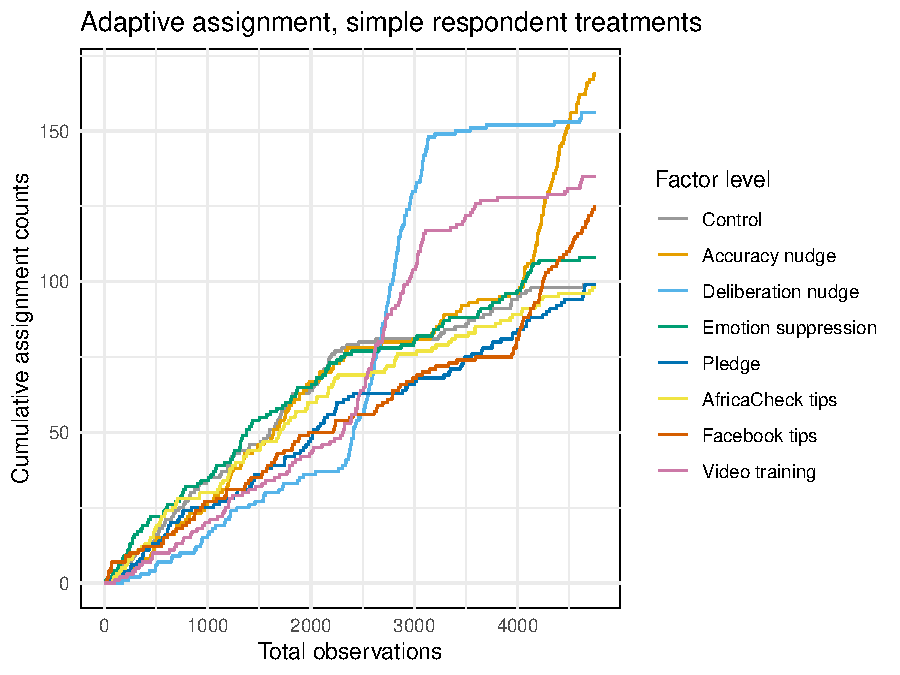
\includegraphics[width = 0.95\textwidth]{../analysis/figures/respondent_base_assignment_on_time.pdf}
    \end{subfigure}%
    \begin{subfigure}[b]{0.5\textwidth}
        \centering
        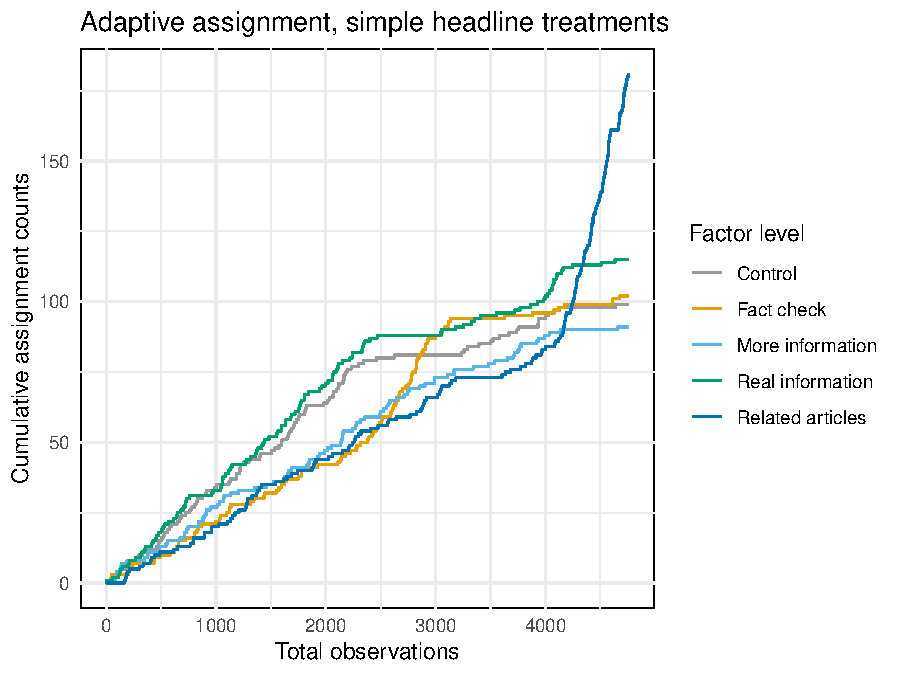
\includegraphics[width = 0.95\textwidth]{../analysis/figures/headline_base_assignment_on_time.pdf}
    \end{subfigure}
   \caption{\textbf{Cumulative treatment assignment during the learning phase for headline (left panel) and respondent (right panel) interventions.} While the full design allows for all factor combinations, these plots illustrate assignment using the ``pure'' version of each factor, i.e., when the other factor is at the baseline control condition.}
   \label{fig:learning_cumulative}
\end{figure}\todo{show something about the bayesian posteriors too?}


This means that we collect more data about the interventions that are the most likely to succeed. It is important to note that adaptively collected data introduces additional challenges for policy learning \citep{zhan2021policy}; the exploitation of the bandit can eventually result in extreme probabilities of treatment assignment. However, this exploitation is an important ethical consideration in a setting where we are concerned about avoiding ``backfire'' from counter-productive interventions. The adaptive algorithm allows us to minimize these potentially harmful effects. %(Figure S4 shows that our adaptive design achieves lower regret compared to a standard static experimental design.)

\begin{figure}[H]
\centering
\textcolor{red}{[TK]}
   \caption{Learning stage estimates grid}
   \label{fig:learning_estimates}
\end{figure}\todo{Add this grid}



\subsection{Evaluation stage}\label{appendix:evaluation}

\newpage

\begin{table}[H]
\small
   \centering
\resizebox{\textwidth}{!}{ 
\begin{tabular}{lccccccc}
&    & \multicolumn{3}{c}{\textbf{False}} & \multicolumn{3}{c}{\textbf{True}} \\
& \textbf{Combined}& Any sharing & Messenger & Timeline & Any sharing & Messenger & Timeline \\
 \cmidrule(lr){2-2}  \cmidrule(lr){3-5}  \cmidrule(lr){6-8}
\multicolumn{4}{l}{\textbf{Age}} \rule{0pt}{1.2\normalbaselineskip} \\														
\hspace{1em} Below median	&	\num{0.022}	&	\num{-0.018}	&	\num{-0.024}+	&	\num{-0.021}	&	\num{-0.022}	&	\num{-0.018}	&	\num{-0.028}*\\
\hspace{1.5em} (n = 5,412)	&	(\num{0.042})	&	(\num{0.014})	&	(\num{0.014})	&	(\num{0.013})	&	(\num{0.015})	&	(\num{0.015})	&	(\num{0.014})\\
\hspace{1em} Above median	&	\num{0.099}*	&	\num{-0.020}	&	\num{-0.015}	&	\num{-0.028}*	&	\num{0.020}	&	\num{0.028}+	&	\num{0.008}\\
\hspace{1.5em} (n = 5,271)	&	(\num{0.047})	&	(\num{0.014})	&	(\num{0.014})	&	(\num{0.014})	&	(\num{0.014})	&	(\num{0.015})	&	(\num{0.014})\\
\cmidrule(lr){2-8}														
\hspace{1em} Difference	&	\num{0.077}	&	\num{-0.001}	&	\num{0.008}	&	\num{-0.007}	&	\num{0.041}*	&	\num{0.046}*	&	\num{0.036}+\\
\hspace{1.5em}	&	(\num{0.064})	&	(\num{0.020})	&	(\num{0.020})	&	(\num{0.019})	&	(\num{0.020})	&	(\num{0.021})	&	(\num{0.020})\\
\multicolumn{4}{l}{\textbf{Gender}}  \rule{0pt}{1.2\normalbaselineskip}\\														
\hspace{1em}Not male	&	\num{0.037}	&	\num{-0.010}	&	\num{-0.017}	&	\num{-0.014}	&	\num{-0.014}	&	\num{0.007}	&	\num{-0.023}\\
\hspace{1.5em} (n = 5,050)	&	(\num{0.045})	&	(\num{0.015})	&	(\num{0.014})	&	(\num{0.013})	&	(\num{0.015})	&	(\num{0.015})	&	(\num{0.015})\\
\hspace{1em} Male	&	\num{0.079}+	&	\num{-0.026}+	&	\num{-0.022}	&	\num{-0.035}*	&	\num{0.010}	&	\num{0.003}	&	\num{0.000}\\
\hspace{1.5em}  (n = 5,633)	&	(\num{0.045})	&	(\num{0.014})	&	(\num{0.014})	&	(\num{0.014})	&	(\num{0.014})	&	(\num{0.014})	&	(\num{0.014})\\
\cmidrule(lr){2-8}														
\hspace{1em} Difference	&	\num{0.042}	&	\num{-0.016}	&	\num{-0.016}	&	\num{-0.016}	&	\num{0.024}	&	\num{0.024}	&	\num{0.024}\\
\hspace{1.5em}	&	(\num{0.063})	&	(\num{0.020})	&	(\num{0.020})	&	(\num{0.020})	&	(\num{0.020})	&	(\num{0.020})	&	(\num{0.020})\\
\multicolumn{4}{l}{\textbf{Political allegiance}} \rule{0pt}{1.2\normalbaselineskip}\\														
\hspace{1em} Not aligned	&	\num{0.102}**	&	\num{-0.029}*	&	\num{-0.028}*	&	\num{-0.035}**	&	\num{-0.002}	&	\num{0.008}	&	\num{-0.008}\\
\hspace{1.5em} (n = 7,570)	&	(\num{0.038})	&	(\num{0.012})	&	(\num{0.012})	&	(\num{0.011})	&	(\num{0.012})	&	(\num{0.012})	&	(\num{0.012})\\
\hspace{1em} Aligned	&	\num{-0.043}	&	\num{0.006}	&	\num{0.001}	&	\num{0.001}	&	\num{0.001}	&	\num{-0.003}	&	\num{-0.017}\\
\hspace{1.5em} (n = 3,113)	&	(\num{0.058})	&	(\num{0.019})	&	(\num{0.018})	&	(\num{0.018})	&	(\num{0.019})	&	(\num{0.019})	&	(\num{0.018})\\
\cmidrule(lr){2-8}														
\hspace{1em} Difference	&	\num{-0.145}*	&	\num{0.035}	&	\num{0.035}	&	\num{0.035}	&	\num{0.004}	&	\num{0.004}	&	\num{0.004}\\
\hspace{1.5em}	&	(\num{0.070})	&	(\num{0.022})	&	(\num{0.022})	&	(\num{0.022})	&	(\num{0.022})	&	(\num{0.022})	&	(\num{0.022})\\
\multicolumn{4}{l}{\textbf{Digital literacy index }}  \rule{0pt}{1.2\normalbaselineskip}\\														
\hspace{1em} Below median	&	\num{0.065}	&	\num{-0.036}*	&	\num{-0.033}*	&	\num{-0.036}**	&	\num{-0.017}	&	\num{-0.006}	&	\num{-0.020}\\
\hspace{1.5em}  (n = 5,443)	&	(\num{0.045})	&	(\num{0.014})	&	(\num{0.014})	&	(\num{0.014})	&	(\num{0.014})	&	(\num{0.014})	&	(\num{0.014})\\
\hspace{1em} Above median	&	\num{0.054}	&	\num{-0.001}	&	\num{-0.006}	&	\num{-0.013}	&	\num{0.016}	&	\num{0.016}	&	\num{-0.001}\\
\hspace{1.5em} (n = 5,240)	&	(\num{0.045})	&	(\num{0.014})	&	(\num{0.014})	&	(\num{0.013})	&	(\num{0.015})	&	(\num{0.015})	&	(\num{0.015})\\
\cmidrule(lr){2-8}														
\hspace{1em} Difference	&	\num{-0.010}	&	\num{0.036}+	&	\num{0.027}	&	\num{0.023}	&	\num{0.033}	&	\num{0.022}	&	\num{0.019}\\
\hspace{1.5em}	&	(\num{0.064})	&	(\num{0.020})	&	(\num{0.020})	&	(\num{0.019})	&	(\num{0.020})	&	(\num{0.021})	&	(\num{0.020})\\
\multicolumn{4}{l}{\textbf{Scientific knowledge index }}  \rule{0pt}{1.2\normalbaselineskip}\\														
\hspace{1em}   Below median	&	\num{0.126}**	&	\num{-0.036}*	&	\num{-0.043}**	&	\num{-0.042}**	&	\num{-0.018}	&	\num{-0.004}	&	\num{-0.030}*\\
\hspace{1.5em} (n = 5,677)	&	(\num{0.043})	&	(\num{0.014})	&	(\num{0.014})	&	(\num{0.013})	&	(\num{0.014})	&	(\num{0.014})	&	(\num{0.014})\\
\hspace{1em}   Above median	&	\num{-0.015}	&	\num{0.000}	&	\num{0.007}	&	\num{-0.005}	&	\num{0.018}	&	\num{0.015}	&	\num{0.012}\\
\hspace{1.5em}  (n = 5,006)	&	(\num{0.047})	&	(\num{0.015})	&	(\num{0.014})	&	(\num{0.014})	&	(\num{0.015})	&	(\num{0.015})	&	(\num{0.015})\\
\cmidrule(lr){2-8}														
\hspace{1em}   Difference	&	\num{-0.141}*	&	\num{0.036}+	&	\num{0.050}*	&	\num{0.037}+	&	\num{0.037}+	&	\num{0.018}	&	\num{0.042}*\\
\hspace{1.5em}	&	(\num{0.064})	&	(\num{0.020})	&	(\num{0.020})	&	(\num{0.019})	&	(\num{0.020})	&	(\num{0.021})	&	(\num{0.020})\\
    \end{tabular}
   }
   \caption{\textbf{Heterogeneity in treatment effects under accuracy nudge by selected covariates.} Estimates are of treatment effects under the accuracy nudge, in contrast with the control condition. Estimates are produced from an augmented inverse probability weighted estimator, as described in Section~\ref{section:estimation}, within specified subgroups. Under two-sided hypothesis tests: \textsuperscript{+} $p<0.1$, \textsuperscript{*} $p < 0.05$, \textsuperscript{**} $p < 0.01$, \textsuperscript{***} $p < 0.001$.}
  \label{tab:heterogeneity_treatment_accuracy}
\end{table}



\begin{table}[H]
\small
   \centering
\resizebox{\textwidth}{!}{ 
\begin{tabular}{lccccccc}
&    & \multicolumn{3}{c}{\textbf{False}} & \multicolumn{3}{c}{\textbf{True}} \\
& \textbf{Combined}& Any sharing & Messenger & Timeline & Any sharing & Messenger & Timeline \\
 \cmidrule(lr){2-2}  \cmidrule(lr){3-5}  \cmidrule(lr){6-8}
\multicolumn{4}{l}{\textbf{Age}} \rule{0pt}{1.2\normalbaselineskip} \\														
\hspace{1em} Below median	&	\num{-0.017}	&	\num{-0.019}	&	\num{-0.018}	&	\num{-0.012}	&	\num{-0.031}+	&	\num{-0.022}	&	\num{-0.040}*\\
\hspace{1.5em} (n = 5,412)	&	(\num{0.046})	&	(\num{0.016})	&	(\num{0.015})	&	(\num{0.014})	&	(\num{0.016})	&	(\num{0.016})	&	(\num{0.016})\\
\hspace{1em} Above median	&	\num{0.110}*	&	\num{-0.044}**	&	\num{-0.045}**	&	\num{-0.042}**	&	\num{-0.002}	&	\num{0.013}	&	\num{-0.003}\\
\hspace{1.5em} (n = 5,271)	&	(\num{0.053})	&	(\num{0.016})	&	(\num{0.016})	&	(\num{0.015})	&	(\num{0.016})	&	(\num{0.016})	&	(\num{0.016})\\
\cmidrule(lr){2-8}														
\hspace{1em} Difference	&	\num{0.127}+	&	\num{-0.025}	&	\num{-0.027}	&	\num{-0.030}	&	\num{0.029}	&	\num{0.034}	&	\num{0.037}\\
\hspace{1.5em}	&	(\num{0.070})	&	(\num{0.022})	&	(\num{0.022})	&	(\num{0.021})	&	(\num{0.023})	&	(\num{0.023})	&	(\num{0.023})\\
\multicolumn{4}{l}{\textbf{Gender}}  \rule{0pt}{1.2\normalbaselineskip}\\														
\hspace{1em}Not male	&	\num{0.038}	&	\num{-0.029}+	&	\num{-0.030}+	&	\num{-0.027}+	&	\num{-0.036}*	&	\num{-0.014}	&	\num{-0.037}*\\
\hspace{1.5em} (n = 5,050)	&	(\num{0.050})	&	(\num{0.016})	&	(\num{0.016})	&	(\num{0.015})	&	(\num{0.017})	&	(\num{0.017})	&	(\num{0.017})\\
\hspace{1em} Male	&	\num{0.053}	&	\num{-0.034}*	&	\num{-0.031}*	&	\num{-0.027}+	&	\num{0.001}	&	\num{0.003}	&	\num{-0.007}\\
\hspace{1.5em}  (n = 5,633)	&	(\num{0.050})	&	(\num{0.015})	&	(\num{0.015})	&	(\num{0.015})	&	(\num{0.015})	&	(\num{0.016})	&	(\num{0.016})\\
\cmidrule(lr){2-8}														
\hspace{1em} Difference	&	\num{0.016}	&	\num{-0.006}	&	\num{-0.006}	&	\num{-0.006}	&	\num{0.037}	&	\num{0.037}	&	\num{0.037}\\
\hspace{1.5em}	&	(\num{0.070})	&	(\num{0.022})	&	(\num{0.022})	&	(\num{0.022})	&	(\num{0.023})	&	(\num{0.023})	&	(\num{0.023})\\
\multicolumn{4}{l}{\textbf{Political allegiance}} \rule{0pt}{1.2\normalbaselineskip}\\														
\hspace{1em} Not aligned	&	\num{0.087}*	&	\num{-0.039}**	&	\num{-0.032}*	&	\num{-0.042}***	&	\num{-0.013}	&	\num{-0.001}	&	\num{-0.019}\\
\hspace{1.5em} (n = 7,570)	&	(\num{0.042})	&	(\num{0.013})	&	(\num{0.013})	&	(\num{0.012})	&	(\num{0.014})	&	(\num{0.014})	&	(\num{0.014})\\
\hspace{1em} Aligned	&	\num{-0.055}	&	\num{-0.015}	&	\num{-0.027}	&	\num{0.010}	&	\num{-0.024}	&	\num{-0.013}	&	\num{-0.027}\\
\hspace{1.5em} (n = 3,113)	&	(\num{0.065})	&	(\num{0.021})	&	(\num{0.020})	&	(\num{0.020})	&	(\num{0.020})	&	(\num{0.021})	&	(\num{0.021})\\
\cmidrule(lr){2-8}														
\hspace{1em} Difference	&	\num{-0.143}+	&	\num{0.024}	&	\num{0.024}	&	\num{0.024}	&	\num{-0.011}	&	\num{-0.011}	&	\num{-0.011}\\
\hspace{1.5em}	&	(\num{0.078})	&	(\num{0.024})	&	(\num{0.024})	&	(\num{0.024})	&	(\num{0.024})	&	(\num{0.024})	&	(\num{0.024})\\
\multicolumn{4}{l}{\textbf{Digital literacy index }}  \rule{0pt}{1.2\normalbaselineskip}\\														
\hspace{1em} Below median	&	\num{0.048}	&	\num{-0.046}**	&	\num{-0.046}**	&	\num{-0.034}*	&	\num{-0.032}*	&	\num{-0.015}	&	\num{-0.033}*\\
\hspace{1.5em}  (n = 5,443)	&	(\num{0.050})	&	(\num{0.016})	&	(\num{0.015})	&	(\num{0.015})	&	(\num{0.015})	&	(\num{0.016})	&	(\num{0.015})\\
\hspace{1em} Above median	&	\num{0.043}	&	\num{-0.017}	&	\num{-0.016}	&	\num{-0.019}	&	\num{0.000}	&	\num{0.006}	&	\num{-0.009}\\
\hspace{1.5em} (n = 5,240)	&	(\num{0.050})	&	(\num{0.016})	&	(\num{0.016})	&	(\num{0.014})	&	(\num{0.017})	&	(\num{0.017})	&	(\num{0.017})\\
\cmidrule(lr){2-8}														
\hspace{1em} Difference	&	\num{-0.005}	&	\num{0.030}	&	\num{0.030}	&	\num{0.015}	&	\num{0.032}	&	\num{0.020}	&	\num{0.024}\\
\hspace{1.5em}	&	(\num{0.070})	&	(\num{0.022})	&	(\num{0.022})	&	(\num{0.021})	&	(\num{0.023})	&	(\num{0.023})	&	(\num{0.023})\\
\multicolumn{4}{l}{\textbf{Scientific knowledge index }}  \rule{0pt}{1.2\normalbaselineskip}\\														
\hspace{1em}   Below median	&	\num{0.061}	&	\num{-0.050}**	&	\num{-0.050}**	&	\num{-0.041}**	&	\num{-0.036}*	&	\num{-0.021}	&	\num{-0.036}*\\
\hspace{1.5em} (n = 5,677)	&	(\num{0.048})	&	(\num{0.016})	&	(\num{0.015})	&	(\num{0.015})	&	(\num{0.016})	&	(\num{0.016})	&	(\num{0.016})\\
\hspace{1em}   Above median	&	\num{0.028}	&	\num{-0.011}	&	\num{-0.009}	&	\num{-0.011}	&	\num{0.006}	&	\num{0.013}	&	\num{-0.004}\\
\hspace{1.5em}  (n = 5,006)	&	(\num{0.052})	&	(\num{0.016})	&	(\num{0.016})	&	(\num{0.015})	&	(\num{0.016})	&	(\num{0.016})	&	(\num{0.016})\\
\cmidrule(lr){2-8}														
\hspace{1em}   Difference	&	\num{-0.033}	&	\num{0.038}+	&	\num{0.041}+	&	\num{0.030}	&	\num{0.042}+	&	\num{0.034}	&	\num{0.032}\\
\hspace{1.5em}	&	(\num{0.071})	&	(\num{0.022})	&	(\num{0.022})	&	(\num{0.021})	&	(\num{0.023})	&	(\num{0.023})	&	(\num{0.023})\\
    \end{tabular}
   }
   \caption{\textbf{Heterogeneity in treatment effects under Facebook tips by selected covariates.} Estimates are of treatment effects under the Facebook tips, in contrast with the control condition. Estimates are produced from an augmented inverse probability weighted estimator, as described in Section~\ref{section:estimation}, within specified subgroups. Under two-sided hypothesis tests: \textsuperscript{+} $p<0.1$, \textsuperscript{*} $p < 0.05$, \textsuperscript{**} $p < 0.01$, \textsuperscript{***} $p < 0.001$.}
  \label{tab:heterogeneity_treatment_facebook}
\end{table}

\todo{TK: additional results. @Molly suggests we pin down results in main text first, then add additional material here. }
\end{document}